This chapter outlines the methods and techniques employed in the development of a conversational question-answering system designed for PDFs. The chapter is structured as follows: Section \ref{sec:overview} provides an overview of the desired use case, its objectives, and constraints concerning a Conversational Question Answering System. Section \ref{sec:conrag} presents a general framework that can be utilized as a decision tree for the practical implementation of a Conversational Question Answering System for PDFs. Its subsections will highlight and discuss the components introduced within the framework.

\section{Overview and Objective}
\label{sec:overview}

The primary use case addressed in this thesis can be summarized as follows: Imagine having a collection of PDF files, and our goal is to create a chatbot capable of engaging in conversations about the knowledge within these PDFs. This chatbot should provide accurate answers to questions based on the content of the PDFs and furnish supporting evidence from these documents. Furthermore, it should enable users to have a conversational query experience, allowing them to ask follow-up questions and engage in dialogue with the chatbot based on its previous responses. Figure \ref{fig:use-case} illustrates an example of this use case.

\begin{figure}
    \centering
    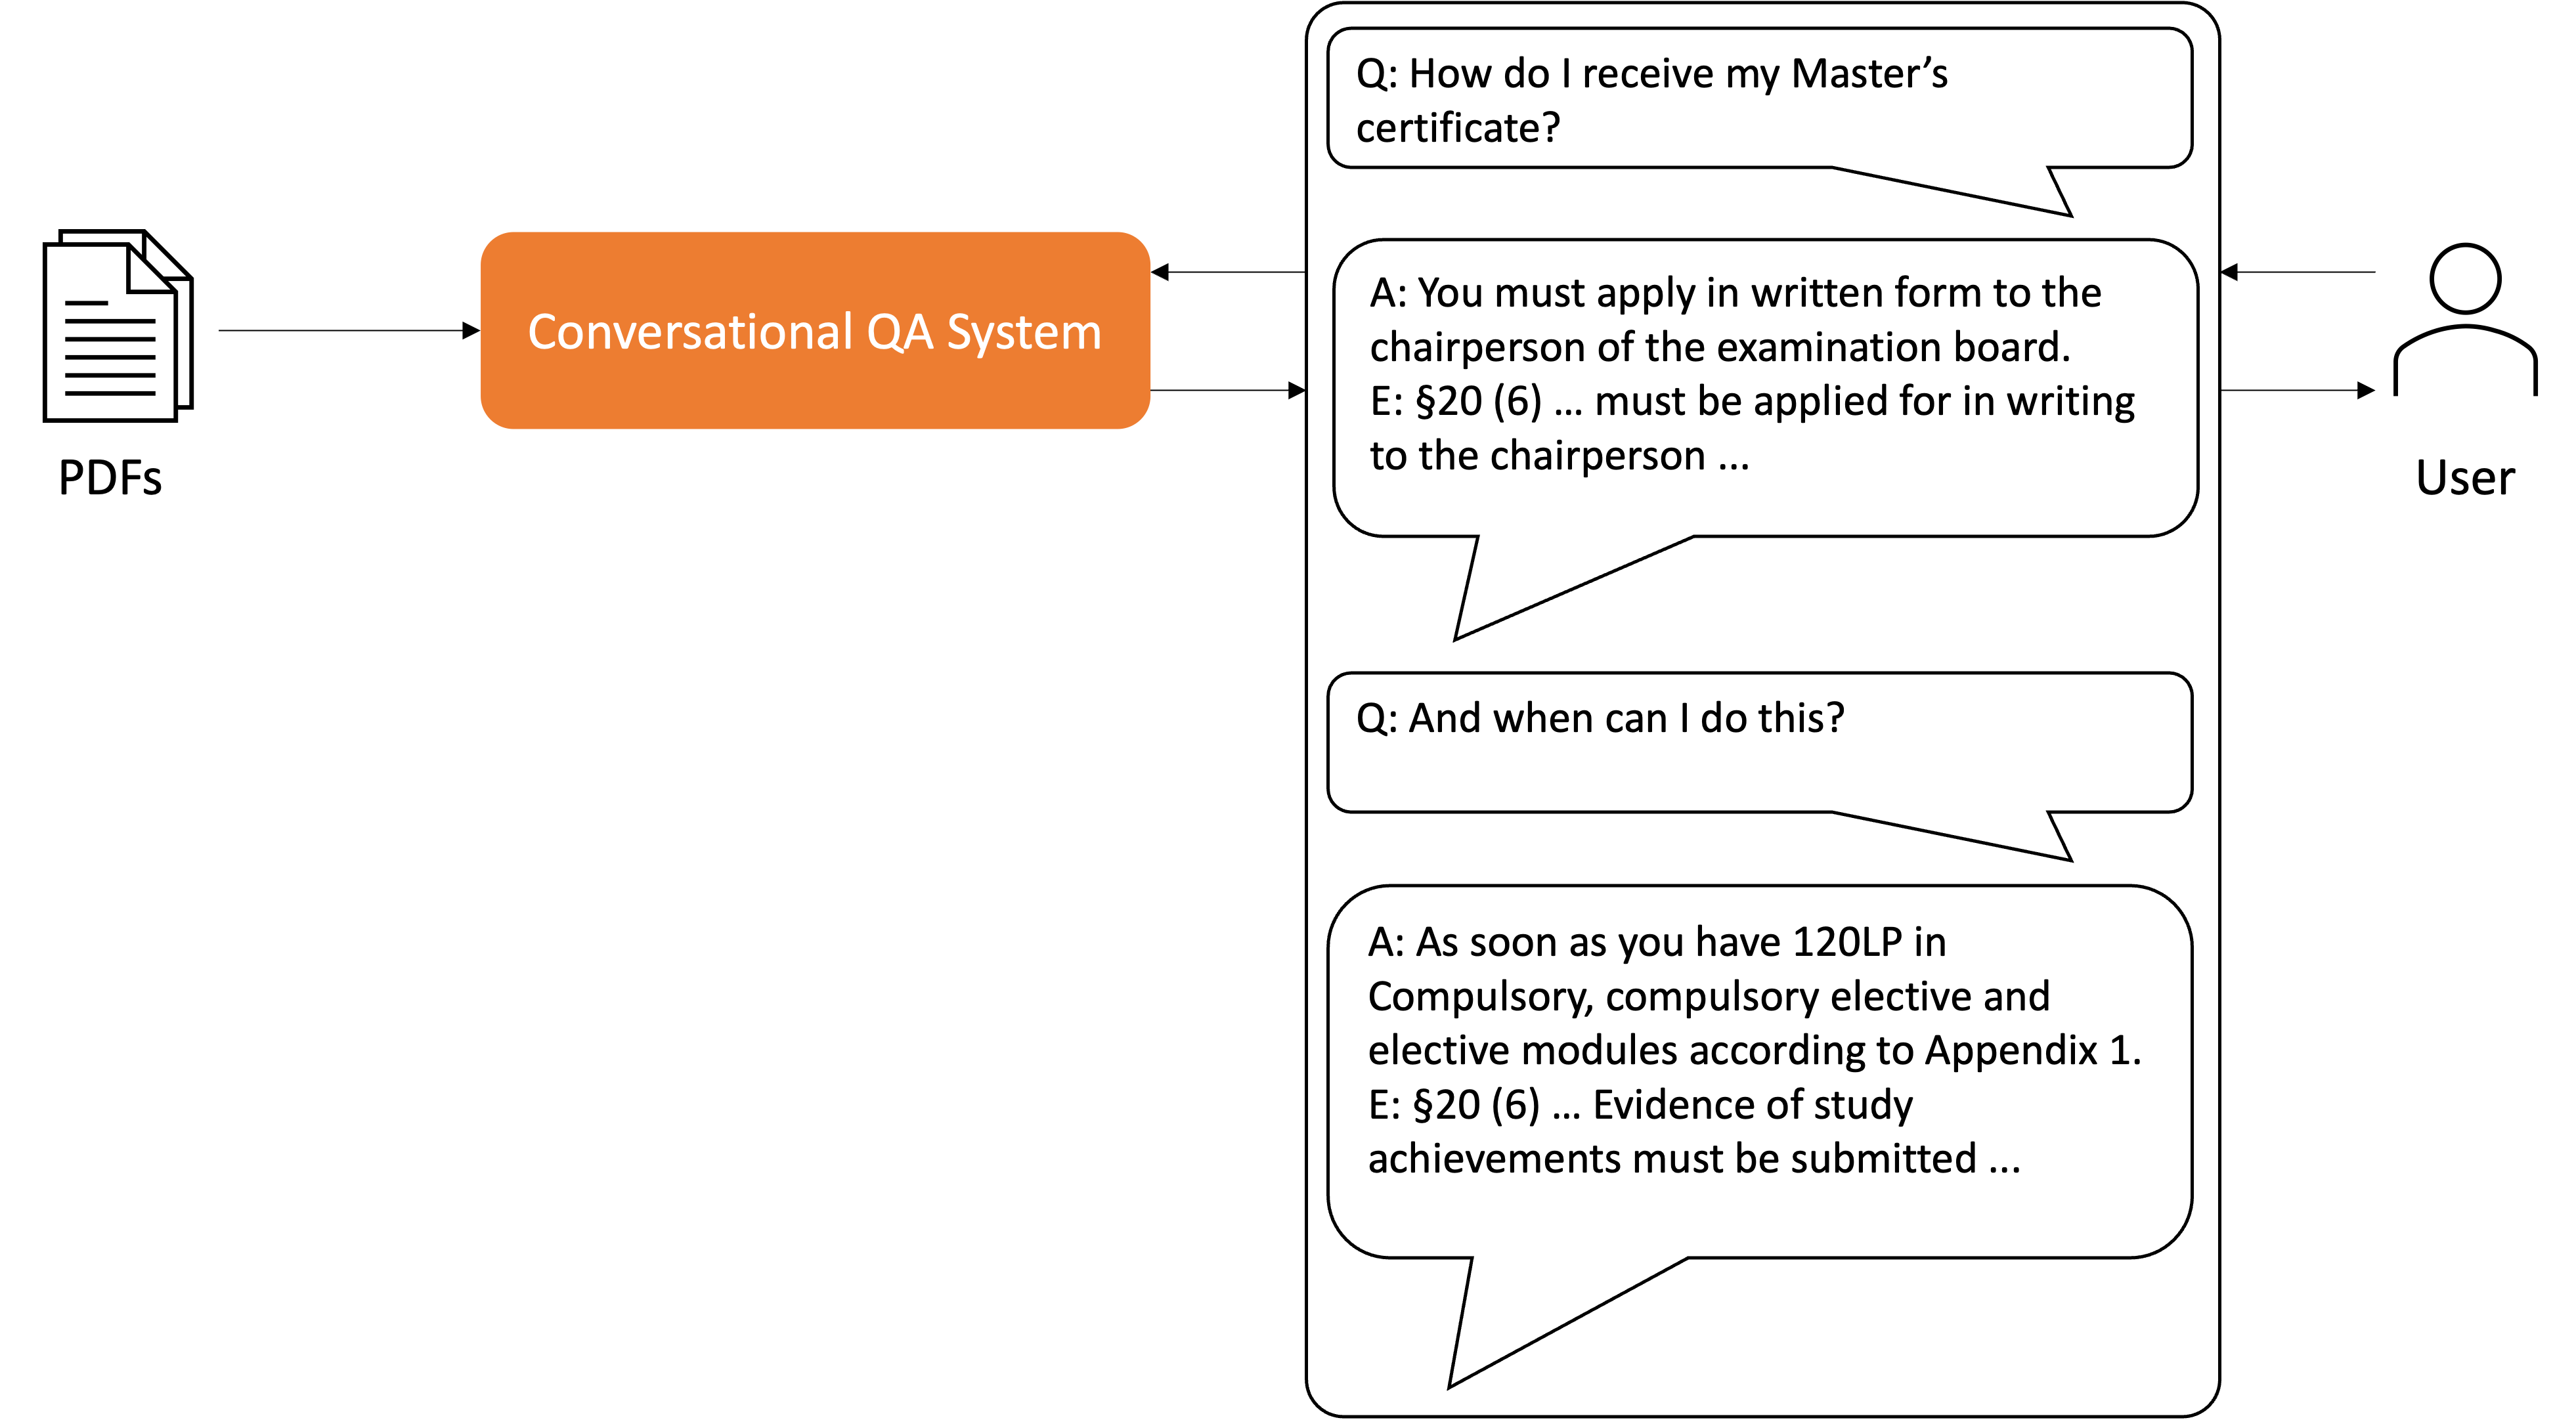
\includegraphics[width=0.8\textwidth]{Grafiken/Use_Case.png}
    \caption{Overview of the Example Use-Case}
    \label{fig:use-case}
\end{figure}

Currently, to the best of my knowledge, there is no scientific paper or similar resource offering a comprehensive framework or pipeline to address this use case. This thesis aims to bridge this gap by presenting a framework and pipeline designed to tackle this specific scenario. Figure \ref{fig:overview-system-architecture} provides an overview of the system architecture. The system follows the \gls{rag} architecture, as detailed in Section \ref{subsec:qa_retrieval}, which extends the classical Retriever-Reader with a \gls{llm} as a Reader, capable of incorporating parametric knowledge. To extend \gls{rag} to a \gls{convqa}, a \gls{cqu} unit, as introduced in Section \ref{subsec:cqa_contextual_query_understanding}, is essential. This novel architecture will be termed \textbf{\gls{conrag}}. The extraction pipeline will be discussed in Section \ref{subsec:extract}, with its primary tasks being the extraction of passages from the provided set of PDFs, the creation of an index, and the optional generation of synthetic training data. The three major modules comprising the architecture, namely the \textit{Retriever}, \textit{Reader}, and \textit{\gls{cqu}}, will be elaborated in their respective sections: \ref{subsec:retriever}, \ref{subsec:reader}, and \ref{subsec:cqu}.

\begin{figure}
    \centering
    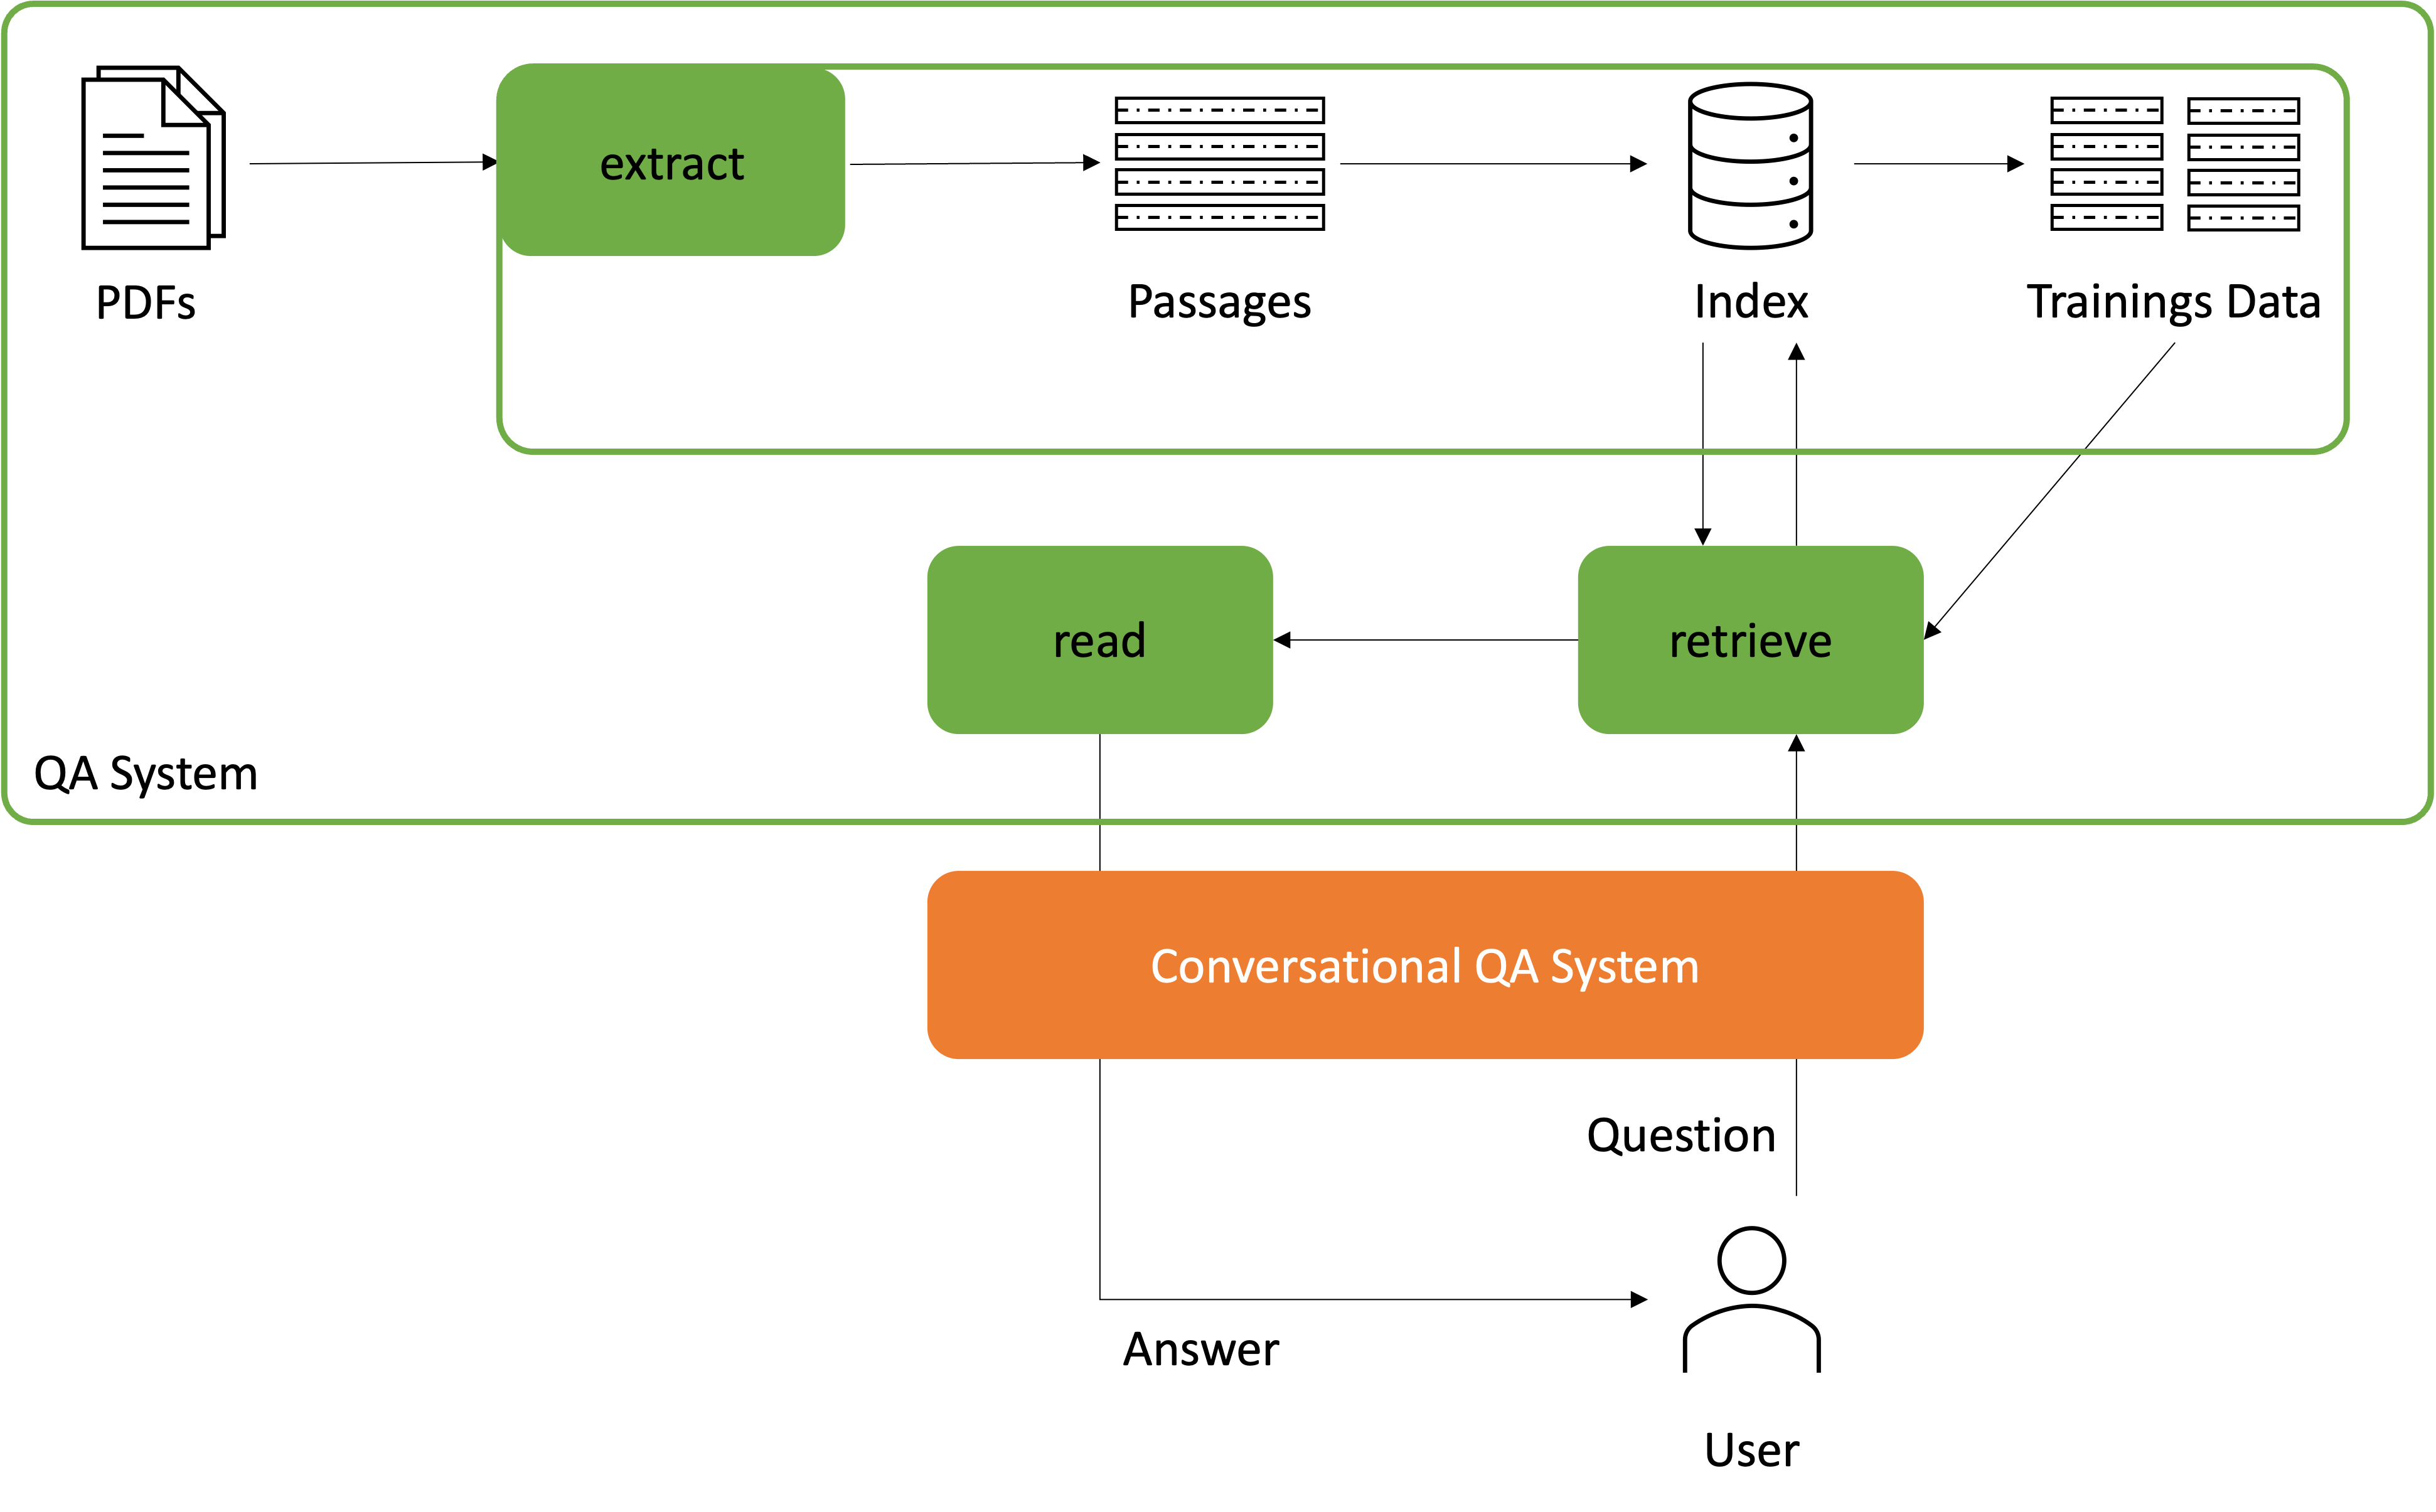
\includegraphics[width=0.8\textwidth]{Grafiken/System_Architecture.png}
    \caption{Overview of the System Architecture}
    \label{fig:overview-system-architecture}
\end{figure}

To summarize, the objectives of the QA capabilities of the system are as follows:

\begin{enumerate}
    \item Utilize \textbf{PDFs} as the primary \textbf{knowledge source}.
    \item Enable the QA-System to handle a \textbf{variety of question types}, including: \textbf{extractive}, \textbf{abstractive}, and \textbf{boolean questions}.
    \item \textbf{Provide references} to PDF snippets \textbf{as evidence to answers}.
    \item Ensure the pipeline's generalizability, allowing it to adapt to new domains or knowledge sources with \textbf{minimal or no supervision} and \textbf{small datasets}.
    \item Design the pipeline to be \textbf{feasible without the need for datacenter-grade hardware resources}, making it accessible for development on standard research hardware.
    \item \textbf{Prioritize accuracy as the primary objective}, as constraining memory consumption is indirectly covered in point (5). \textbf{Latency is not a primary concern}, as the system is not intended for real-time use and will not be optimized for that.
\end{enumerate}


Regarding the ConvQA-System, the objectives are as follows:

\begin{enumerate}
    \item Enable the ConvQA-System to \textbf{handle} the following follow-up \textbf{question types: drilling-down, clarification, topic shift} and \textbf{comparison}.
    \item Be able to take Initiative in the form of \textbf{clarifying questions}.
    \item The \textbf{memory} will be \textbf{limited to a session}.
\end{enumerate}

\section{Problem Statement}
\label{sec:problem_statement}

The following Section will layout the problem of document-based \gls{convqa}. 

Substantially the fundamental thing given, is some sort of \textit{Document}. A \textit{Document} can be any type of structured or unstructured file, which is being used for storing and displaying information. Examples could be HTML (structured) or PDF (unstructured) files. A \textit{Document} consits of content $C_d$, a collection of strings $c_d$, whereas the content $C_d$ has to have at least one $c_d$, but can contain also multiple, a topic $t$, which is an abstract entity and has no finite set of $T$, a topic could be for example \enquote{Examination Regulation of the Master of Data and Computer Science at the University Heidelberg}, and a unique identifier $UID_d$, therefore a \textit{Document} $d = (C_d,t, UID_d)$. For this thesis we will only cosider textual content $C_d$ and not figures or images. Out of the necessity, for knowledge granularity and precise information context, we will define \textit{Passages} next. A \textit{Passage} $p$ is a subset of a textual content strings $c_d \in C_d$. The granularity of $p$ can be defined use-case specific. If $p$ is a sentence, 100 tokens or other depends on the given scenario. Nevertheless, every $p$ contains a reference to the orgianl document $d$ it was taken from and has it's own unique identifier $UID_p$. This leads to the following \textit{Passage Model}:
\begin{definition}
    \textbf{(Passage Model)} A passage $p$ is a subset of a textual content string $c_d \in C_d$ of a document $d = (C_d,t, UID_d)$, whereas $p = (content, UID_p, UID_d)$.
    \label{def:passage_model}
\end{definition}

For the ease of notation, we will refer to the content of a passage $p$ as $p$ itself in the following. The collection of all \textit{Passages} $P$ will be refered to as the \textit{Knowledge Source}. 

Next we need to define what a \textit{Question} is. For this problem, a question consits of a string - $content$, which incorporates a question in natural language and an intent $i \in I$, which also again is an abstract entity, refereing to the actual information need $q$ should fullfill. The \textit{Question Model} can therefore be defined as follows:

\begin{definition}
    \textbf{(Question Model)} A question $q$ is a tuple $(content, i)$, whereas $content$ is a string and $i \in I$.
    \label{def:question_model}
\end{definition}

Also here we will refer to the content of a question $q$ as $q$ itself in the following, for reducing the complexity of the notation.

Naturally given a \textit{Question}, there has to be an \textit{Answer}. An \textit{Answer} $a$ is a string, which is the answer to a \textit{Question} $q$, given that it fullfills the intent $i$ of $q$. This is being refered to as $I(q,a) = 1$. Formally we define an \textit{Answer} as:

\begin{definition}
    \textbf{(Answer Model)} An answer $a$ is a string, which answers a given question $q$ under the condition, that the search intent of $q$ is satisfied $I(q,a) = 1$.
    \label{def:answer_model}
\end{definition}

In terms of conversations, we split an exchange between two agents into \textit{Turns} as described in Section \ref{subsec:cqa_basics}. Generally speaking, a \textit{Turn} $h$ consists of a tuple $(q,a)$, whereas the $a$ is the response to $q$. \textit{Turns} happen in order and have a relation between each other. Therefore we refer to the collection of multiple \textit{Turns} within one conversation as \textit{History} $H$.

\begin{definition}
    \textbf{(History Model)} A history $H$ is a collection of turns $h$, whereas $h = (q,a)$.
    \label{def:history_model}
\end{definition}

As we now have elaborated, what \textit{Questions}, \textit{Knowledge Source}, \textit{Answers} and \textit{History} are, we're ready to define the problem of \gls{convqa}:

\begin{definition}
    \textbf{(Conversational Question Answering Task)} Given a new question $q_{i+1}$ and a history $H$ with $i$-many turns $h$, a model ($M$) should generate an answer $a_{i+1}$, based on the provided knowledge in the knowledge source $P$, which satisfies the search intent $i$ of $q_{i+1}$. Next to the answer $a_{i+1}$, $M$ should return $p$ as evidence from $P$. Formally:
    \begin{align*}
        \mathbf{M: (q_{i+1}, H, P) \rightarrow (a_{i+1}, p)}
    \end{align*}
    \label{def:task}
\end{definition}

\section{Conversational Retrieval-Augmented Generation}
\label{sec:conrag}

In order to provide a solution to the Task of \gls{convqa} as defined in Definition \ref{def:convqa}, the system must be able to perform evidence selection based on a \textit{Knowledge Source} which is an important criterion also layed out in Section \ref{sec:overview}. 

In order to now create a system architecture, which fullfills the task of model $M$ (see Definition \ref{def:task}), we will split the main task of \gls{convqa} into multiple subtasks:

\begin{enumerate}
    \item \textbf{Information Extraction:} Given a set of documents $D$, extract the textual content $C_d$ of each document $d \in D$ and create a knowledge source $P$ based on $C_d$ of every document $d \in D$.
    \item \textbf{Contextual Question Understanding:} Given a history $H$ and a new question $q_{i+1}$, generate a contextualized question $q_c$ based on $H$, sothat $I(q_c,q_{i+1}) = 1$.
    \item \textbf{Passage Retrieval:} Given a contextualized question $q_c$ and a knowledge source $P$, retrieve the $k$-most relevant passages $p$ from $P$ and combine them in an evidence set $E$.
    \item \textbf{Response Generation:} Given a contextualized question $q_c$ and a set of passages $E$, generate an answer $a$ to $q_c$ based on $E$, so that $I(q_{i+1},a) = 1$.
\end{enumerate}

There may exist other approaches to break down the task of $M$ into sub-tasks, but for this thesis, we will focus on a solution based on the four sub-tasks outlined above. The reason is simply the existing state-of-the-art research in every field of this sub-tasks, especially when it comes to the adoption of new domains. It is to be highlighed, that breaking the task of $M$ implies also an order in which the sub-tasks have to be performed. Sub-task (1) will be performed once, while (2-4) will be repeated on every new question $q_{i+1}$.

In order to develop a system which can be applied to this abstract task, we match every task with a component. The \textit{Information Extraction} sub-task will be solved by the \textit{extract} component, further detailed in Section \ref{subsec:extract}. \textit{Passage Retrieval} will be covered by the \textit{Retriever} component, further discribed in Section \ref{subsec:retriever}. The \textit{Response Generation} will be handled by the \textit{Reader} component, more precisely in this thesis we will focus on \gls{llm}s with intrinsic parametric knowledge as \textit{Reader}. This will lead to a \gls{rag} system consisting of the \textit{Retriever} and \textit{Reader}. This choice has been made due to the fact, that the latest reasearch breakthroughs sparked the interest in \gls{rag} systems in compraison towards classical Retriever-Reader systems (check herefore the related work Section \ref{sec:related_work}). Details on the \textit{Reader} component will be layed out in Section \ref{subsec:reader}. In order to now handle conversations, a \gls{cqu} unit as described in Section \ref{subsec:cqa_contextual_query_understanding} is necessary to handle the sub-task of \textit{Contextual Question Understanding}. Section \ref{subsec:cqu} will dive into the details.

\begin{figure}
    \centering
    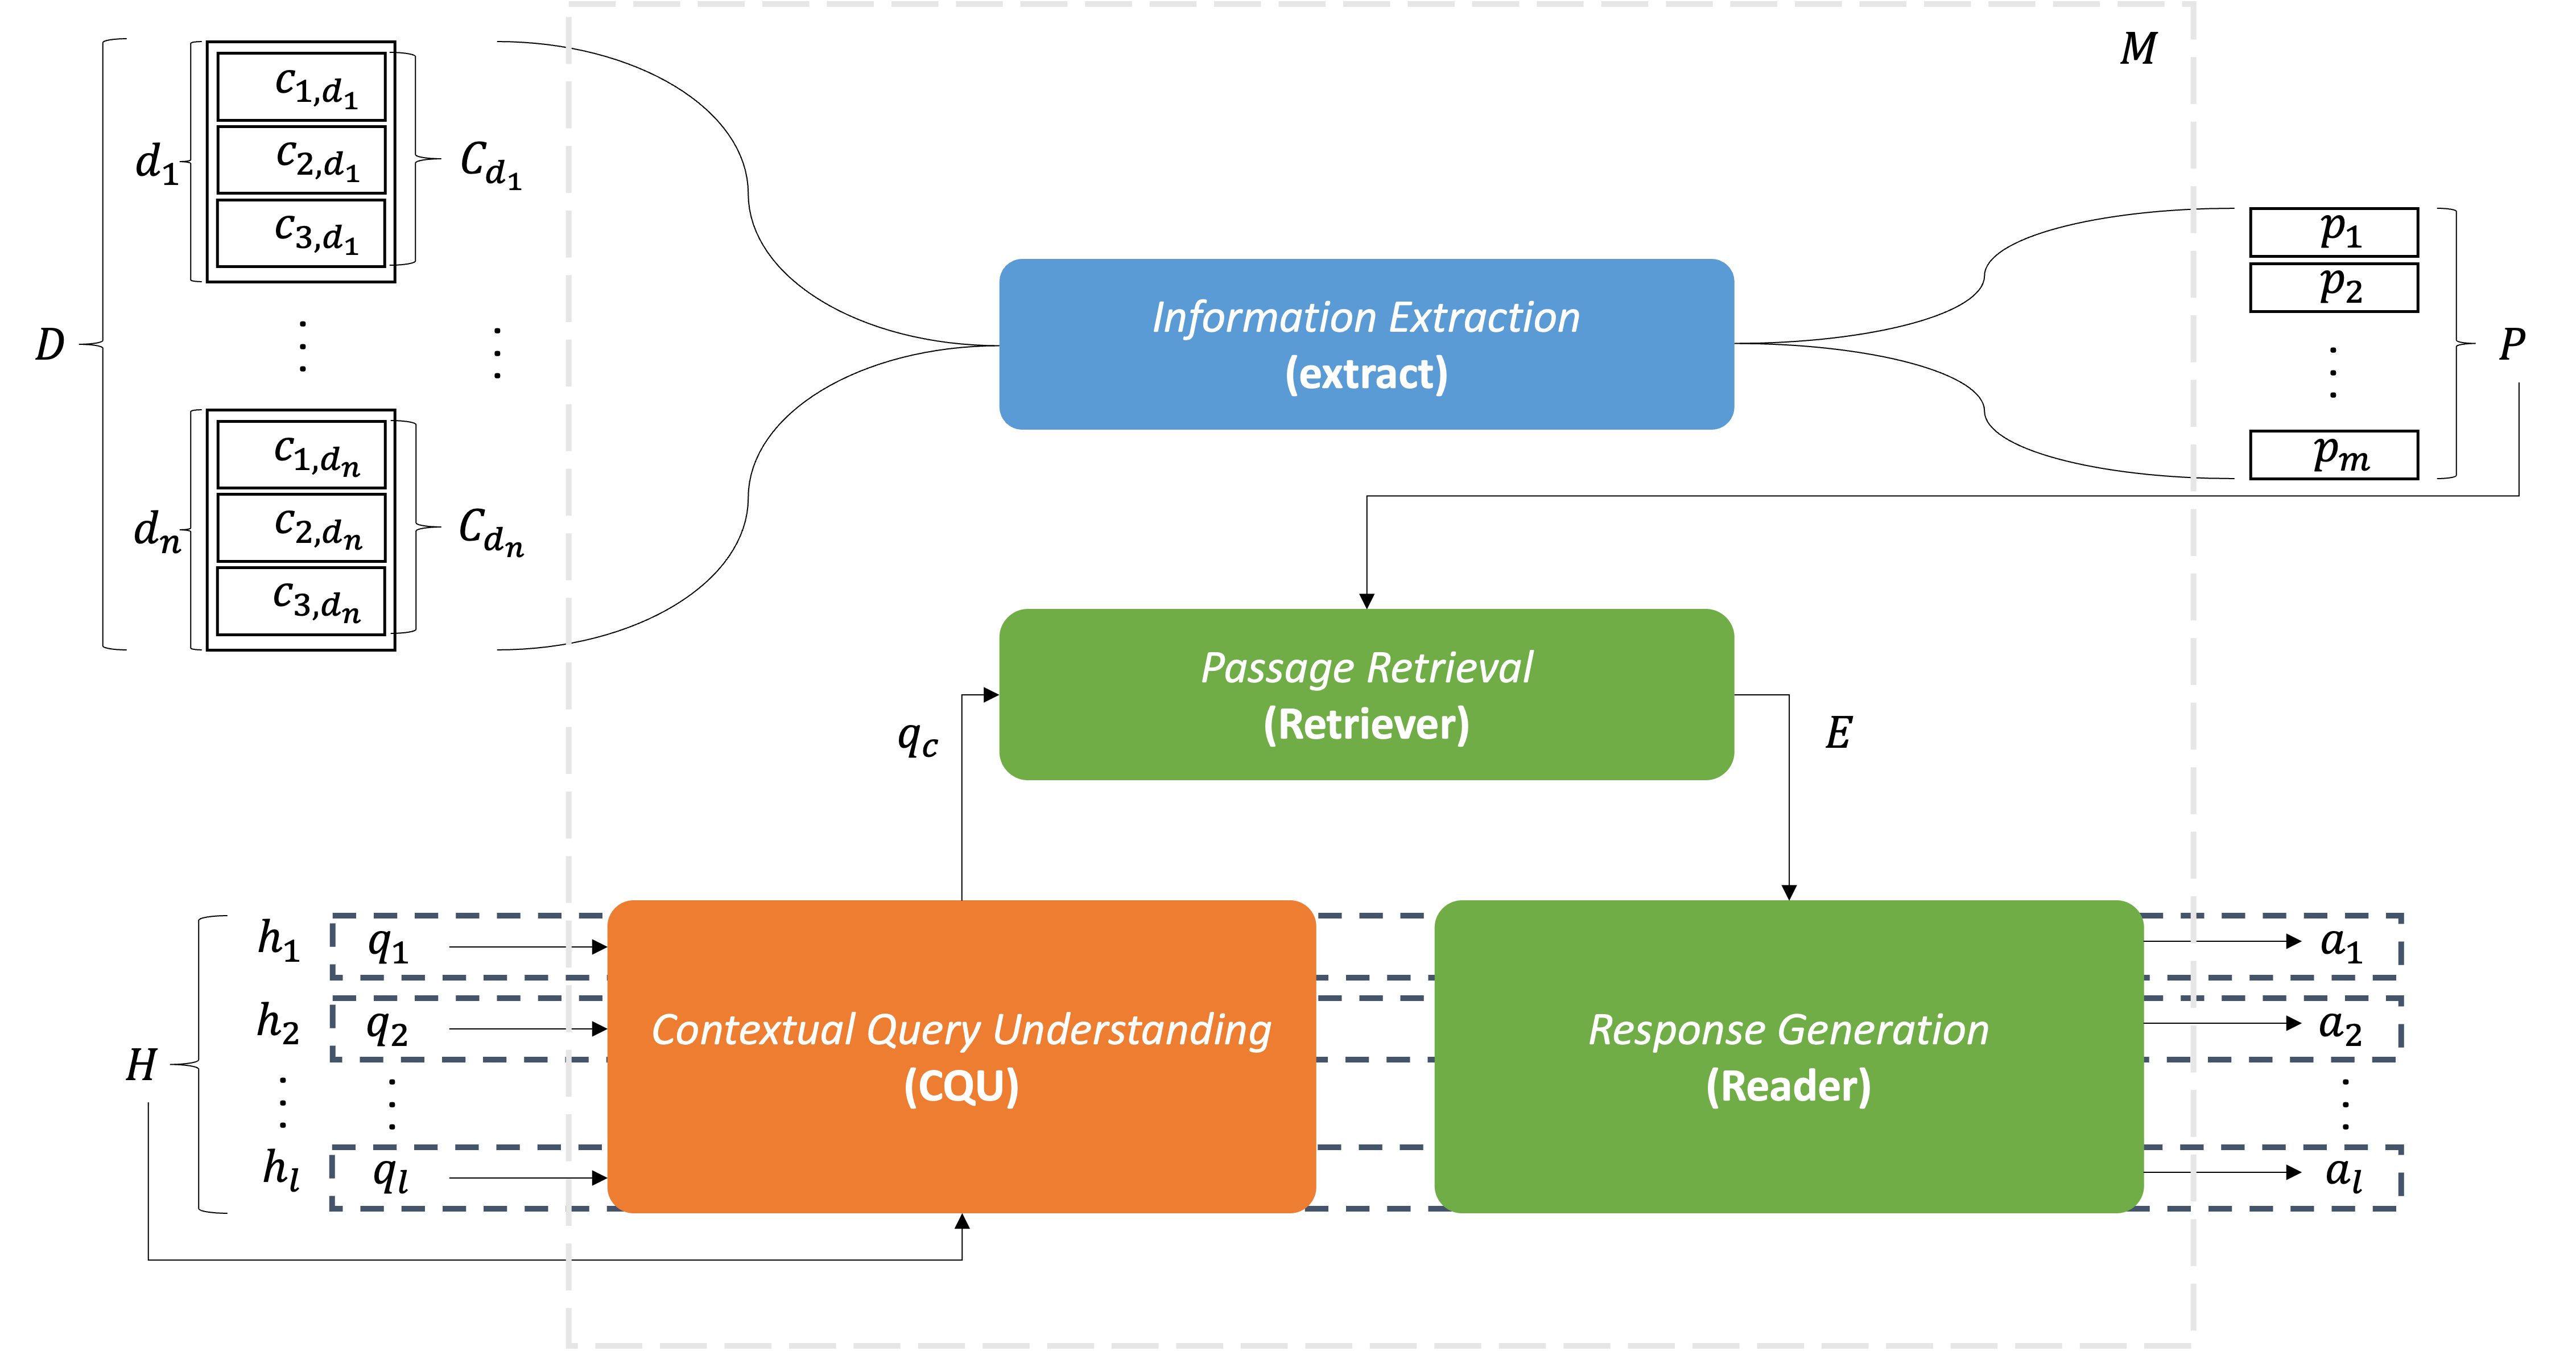
\includegraphics[width=0.8\textwidth]{Grafiken/conrag_konzeptionell.png}
    \caption{Overview of the System Architecture in context of the sub-tasks of $M$}
    \label{fig:conrag_concept_system_architecture}
\end{figure}

Figure \ref{fig:conrag_concept_system_architecture} illustrates the combination of the four components, which make up the model $M$ in their corresponding sub-tasks. This is the abstract Model $M$ which leads, when applied to a real use-case, to the \gls{conrag} system architecture.

% In relation to related work, for some of these sub-tasks, there are already existing components/models, which fullfill this tasks. \textit{Information Extraction} is a well researched field, with many different approaches and models as outlined in Section \ref{subsec:qa_indexing}. Section \ref{subsec:extract} will delve into the details of this sub-task in this context. \textit{Passage Retrieval} and \textit{Response Generation} are commonly implemented as Retriever-Reader Systems as outlined in Section \ref{sec:qa}, nevertheless for this thesis, we will narrow the focus down on \gls{rag} Systems only, as they gained a lot of attention in the last year of research. Details of a both retriever and reader for this specific task will be\textit{Contextual Question Understanding} is a less researched field, with only a few approaches and models.

% This excludes fully generative Models, which can only propose an answer $a$ based on their parametric knowledge. Therefore, the system architecture will have to be based on a Retriever-Reader Architecture. In a Retriever-Reader Architecture, the Retriever identifies important passages $p$ from the knowledge source $P$ given a question $q$ (See Section \ref{subsec:qa_architectures}).

% In the following section, we will outline the general problem field of \gls{convqa}. Unlike other definitions of this problem field, our definition begins with a collection of documents $d \in D$, where \textit{document} refers to any textual knowledge source (e.g., plain text, web pages, etc.). The core task of \gls{convqa} can be defined as follows:

% \begin{definition}
%     \textbf{(\gls{convqa} Task)} The task comprises (i) information extraction, (ii) passage retrieval, (iii) response generation, and (iv) question understanding.
%     \label{def:task}
% \end{definition}

% The system architecture \gls{conrag}, introduced in Section \ref{sec:overview} (see Figure \ref{fig:convqa_system_architecture}), divides these four tasks among four components. Each of these sub-tasks corresponds to a different mechanism of the model ($M$), which is designed to engage in a conversation with a user over a collection of documents $D$. The first task (i) of extraction can be defined as follows:

% \begin{definition}
%     \textbf{(extraction)} An extraction model ($Ext$) is a model which extracts passages from a collection of documents $D$.
%     \begin{align*}
%         \mathbf{Ext: D \rightarrow P}
%     \end{align*} 
%     Whereas $P$ is a set of passages $p \in P$ and $\forall d \in D, \exists p \in P : p \subseteq d$.
%     \label{def:extraction}
% \end{definition}

% Therefore, the input to the next component of $M$, the Retriever $p_\eta(p|q)$, is as follows:

% \begin{equation}
%     \text{Input} = (Q, P) :
%     \begin{cases}
%         \begin{aligned}
%             &\text{question}, && Q = \{q_1, \ldots, q_m\} \\
%             &\text{knowledge source}, && P = \{p_1, \ldots, p_n\}
%         \end{aligned}
%     \end{cases}
% \end{equation}

% This means that the input is a tuple $(Q,P)$ consisting of a set of questions $Q = \{q_1, q_2, \ldots, q_m\}$ and a knowledge source $P = \{p_1, p_2, \ldots, p_n\}$. Therefore, the task of $p_\eta(p|q)$ with parameters $\eta$ can be defined as follows:

% \begin{definition}
%     \textbf{(Passage Retrieval)} A retrieval model ($p_\eta(p|q)$) is a model that generates a relevance score for every tuple $(q,p)$.
%     \begin{align*}
%         \mathbf{p_\eta(p|q) = Score(q,p)}
%     \end{align*}
%     Here, $q$ itself is a tuple $(q,i)$, where $i \in I$, and $I$ is the set of all possible search intents. 
%     \label{def:retrieval}
% \end{definition}

% The set of search intents $I$ (e.g., extractive, abstractive, etc., see Section \ref{subsec:cqa_basics}) is finite. The index $i$ of a question $q$ is implicit and therefore not further specified in the following notations. Hence, instead of representing the whole tuple as $(q,i)$ for each question, we simplify it to just $q$. Task (iii) of response generation is carried out by a generator/reader $p_\theta(a|q,p)$ with parameter $\theta$:

% \begin{definition}
%     \textbf{(Response Generation)} A generation model ($p_\theta(a|q,p)$) is a model that generates an answer $a$ given a question $q$ and top-$k$ retrieved passages $p$.
%     \begin{align*}
%         \mathbf{p_\theta(a|q,p) = a}
%     \end{align*}
%     \label{def:generation}
% \end{definition}

% In a more general context, we assume that there always exists a correct answer $a$ to a question $q$ that can be extracted from the passages $P$. Therefore, we distinguish the following cases:

% \begin{equation}
%     \forall q \in Q, \exists! a \in A : a = 
%     \begin{cases}
%         \begin{aligned}
%             &1. \text{ } f(q, \emptyset), \text{ } &\text{if there is no evidence in } P \\
%             &2. \text{ } f(q, p), \text{ } &\text{if there is exactly one piece of evidence in } P \\
%             &3. \text{ } f(q, E) \mid E \subset P, \text{ } &\text{if there are multiple pieces of evidence in } P
%         \end{aligned}
%     \end{cases}
% \end{equation}

% In case 1, the answer $a$ to the question $q$ indicates that there is no evidence available for this question. Depending on the specific question $q$ intend $i$, this can lead to different answers. Case 2 can be an example of a common extraction question $q$ where the answer $a$ refers to an exact span in one passage $p$. Case 3 involves more complex questions $q$ that require information from multiple passages $p$ to be answered correctly.

% Lastly, task (vi) is handled by a \gls{cqu} $p_\xi(q_c|H,q_i)$ with parameter $\xi$:

% \begin{definition}
%     \textbf{(Question Understanding)} A question understanding model ($p_\xi(q_c|H,q_i)$) is a model that generates a contextualized question $q_c$ given a history $H$.
%     \begin{align*}
%         \mathbf{p_\xi(q_c|H, q_i) = q}
%     \end{align*}
%     Contextualized refers to identifying language-specific features between turns of a conversation to incorporate the context of the conversation into the question $q_i$.
%     \label{def:question_understanding}
% \end{definition}

% The history $H$ is further described in Section \ref{subsec:cqa_basics}.

% Figure \ref{fig:task_convqa} illustrates the general task of \gls{convqa}. It displays the relationship between questions, answers, documents, and the model $M$ on a high level. The following sections will delve deeper into the individual components of $M$. Section \ref{subsec:extract} will discuss sub-task (i), Section \ref{subsec:retriever} will discuss sub-task (ii), Section \ref{subsec:reader} will focus on sub-task (iii), and Section \ref{subsec:cqu} will explore sub-task (vi).

% \begin{figure}
%     \centering
%     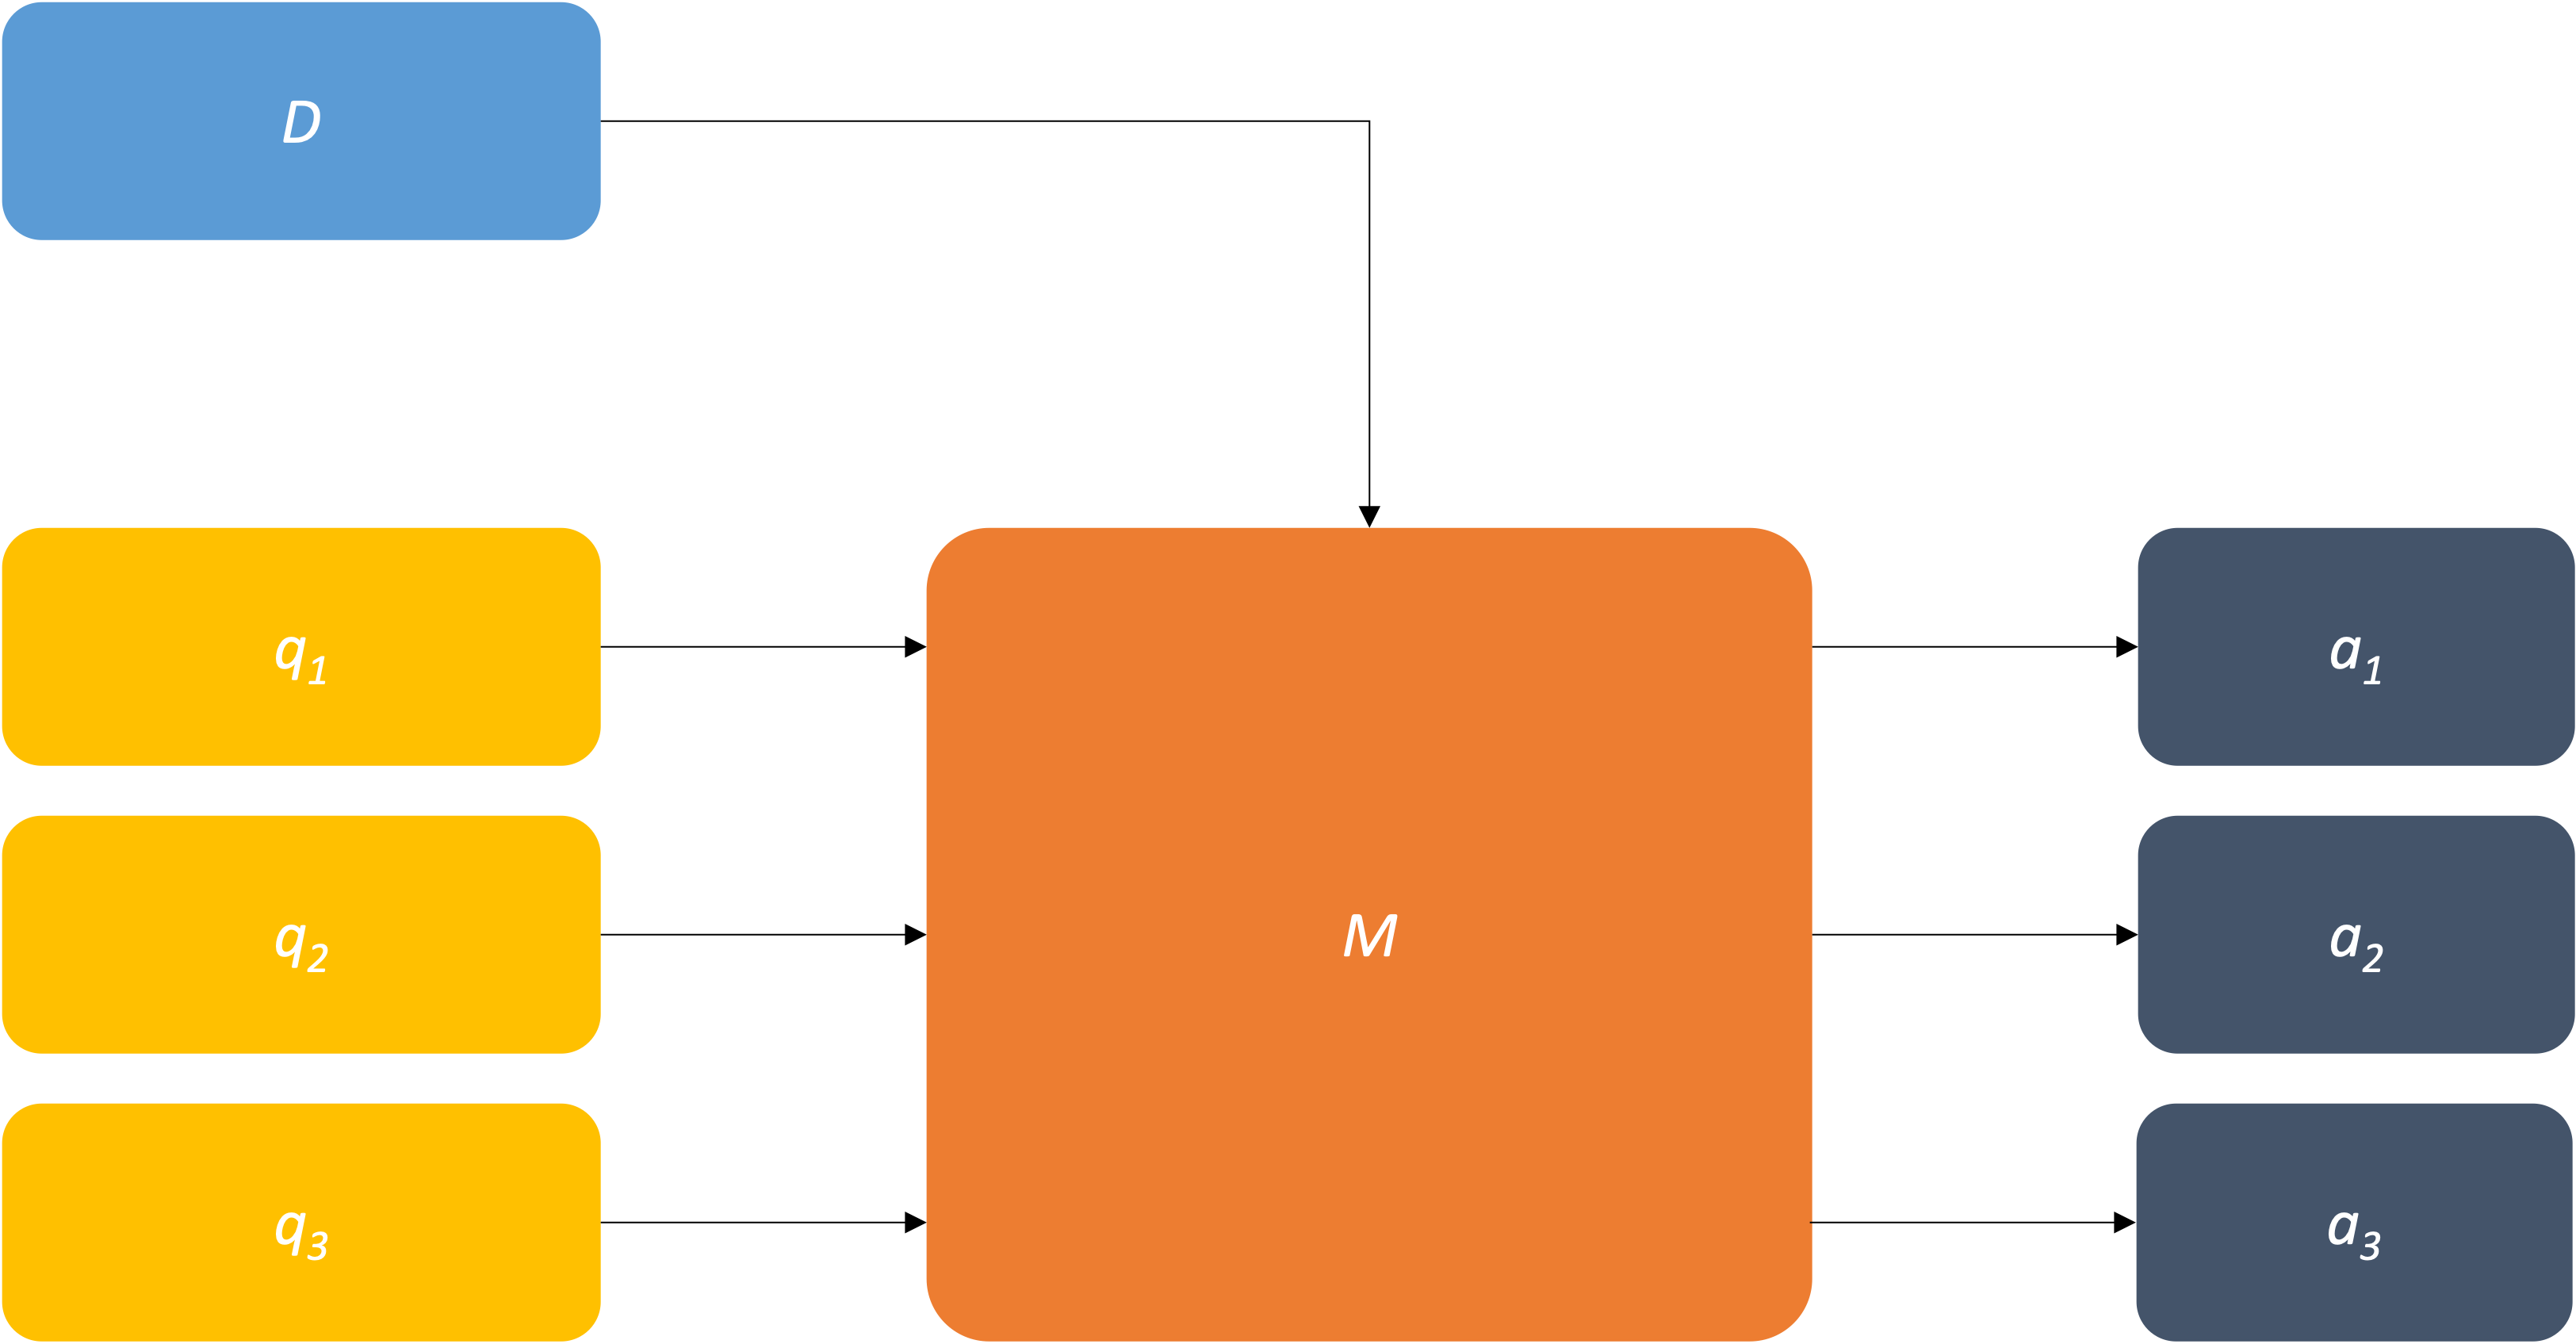
\includegraphics[width=0.8\textwidth]{Grafiken/general_conqa.png}
%     \caption{General Task of \gls{convqa}}
%     \label{fig:task_convqa}
% \end{figure}


% As illustrated in Figure \ref{fig:overview-system-architecture}, it is logical to partition the extensive grid of possibilities into smaller, manageable components that can be explored and designed independently. Consequently, the framework will be divided into two main segments: the extraction pipeline, with its potential configurations outlined in Figure \ref{fig:extract_pipeline}, and the three major modules: Retriever, Reader, and \gls{cqu}, showcasing their possible implementations in Figure \ref{fig:all_components_conrag}.

% \begin{figure}
%     \centering
%     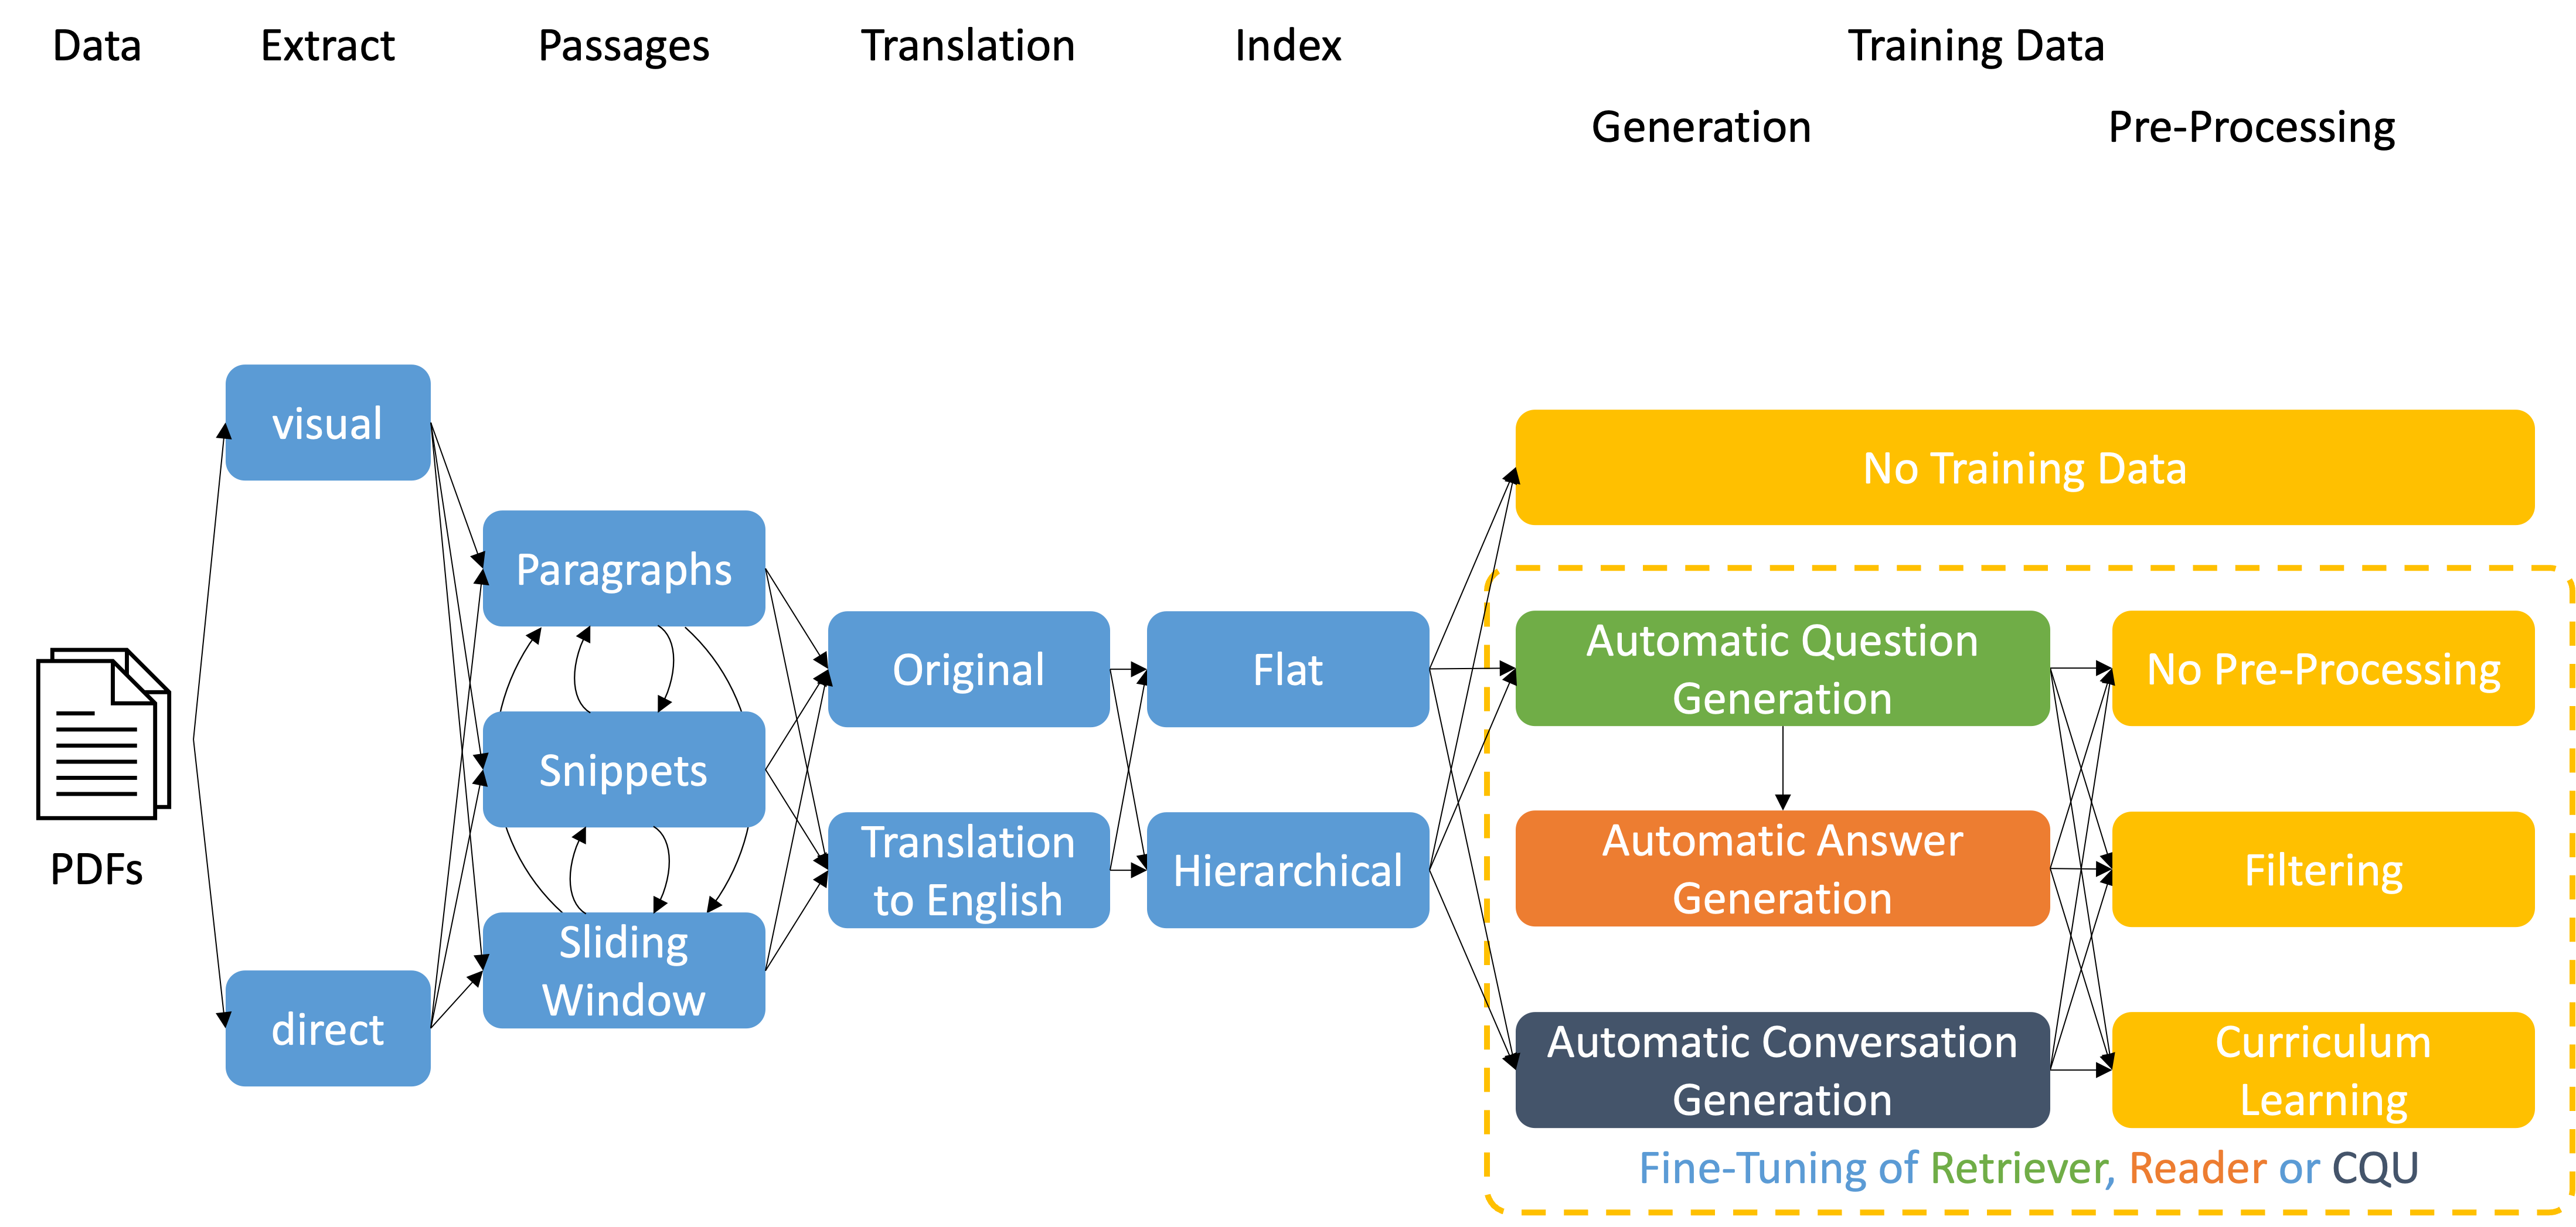
\includegraphics[width=\textwidth]{Grafiken/extract_pipeline.png}
%     \caption{Overview of the Extraction Pipeline Framework}
%     \label{fig:extract_pipeline}
% \end{figure}

% The framework varies in its level of granularity, shifting between high-level concepts and precise details. This is primarily due to the fact that certain aspects of the framework are well-researched and represent state-of-the-art knowledge, while others are ongoing research and necessitate a more abstract, conceptual treatment. For instance, \textit{BM25} is mentioned specifically as the state-of-the-art Sparse Retriever within the Retriever Module, whereas \textit{Automatic Question Generation} in the Training Data Generation step of the extraction pipeline is presented as a high-level concept.

% The framework strives to maintain a high level of generality, intentionally avoiding the incorporation of restrictive paradigms, except for the specified system architecture of \gls{rag} for \gls{qa}. This decision is motivated by the breakthroughs and extensive research endeavors within the field of \gls{llm}s, as exemplified by the exceptional success of \textit{ChatGPT}. In response to the limitations of ChatGPT, including \textit{hallucination}, \textit{implicit knowledge}, and \textit{static knowledge}, interest has surged in the \gls{rag} architecture as a means to address these issues. Presently, there is no existing survey or similar resource that provides a quantitative evaluation of the ongoing business initiatives aimed at implementing RAG-based Systems. Nonetheless, both Google Cloud Services \cite{noauthor_generative_nodate} and Amazon Web Services \cite{noauthor_quickly_2023} have introduced new services that empower customers to construct \gls{rag}-based systems, with Langchain serving as the Framework for the Reader Implementation \cite{noauthor_langchain-ailangchain_nodate}. Consequently, the framework presented here seeks to illuminate potential pathways for implementing a \gls{conrag} system, as depicted in Figure \ref{fig:convqa_system_architecture}, tailored to the use case described in Section \ref{sec:overview}.

% The extraction pipeline can be visualized as a tree, where following different paths signifies making decisions with corresponding implications for subsequent steps and components. In Figure \ref{fig:all_components_conrag}, each column represents a decision to be made, although in some cases, choosing not to decide is itself a decision. Dotted lines encircling multiple frames indicate that a combination or ensemble approach is possible. For a better understanding of how to apply this framework to create a potential system implementation, refer to the example in Figure \ref{fig:example_decission_tree}. As previously mentioned, the framework does not prescribe specific models (e.g., BERT, PaLM, etc.) but rather conceptual approaches (e.g., Cross-Encoder). The example in Figure \ref{fig:example_decission_tree} represents a simple zero-shot baseline, which will also be implemented and tested in this thesis Chapter \ref{chap:eval}.

% \begin{figure}
%     \centering
%     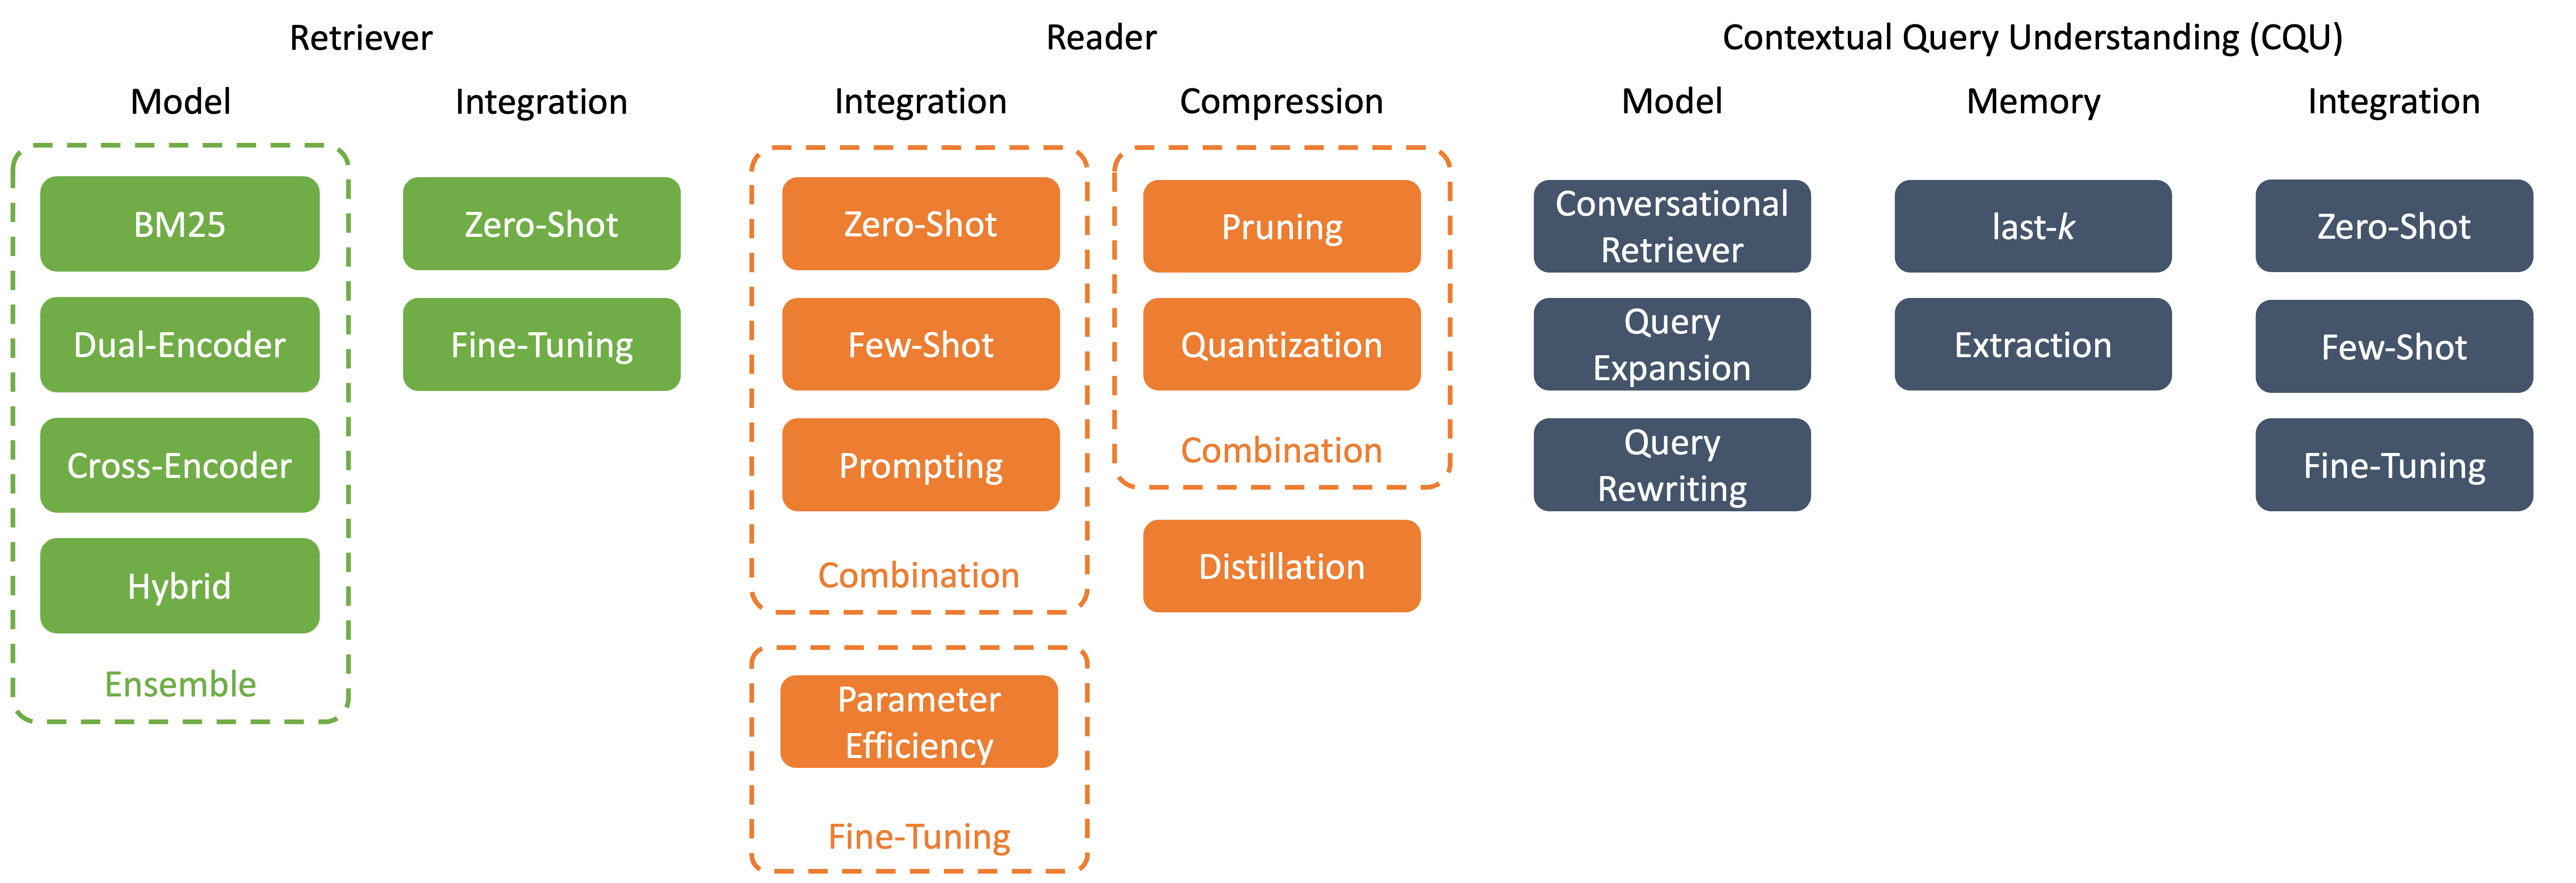
\includegraphics[width=\textwidth]{Grafiken/all_components_conrag.png}
%     \caption{Overview of all Modules of the Framework}
%     \label{fig:all_components_conrag}
% \end{figure}

% \begin{figure}
%     \centering
%     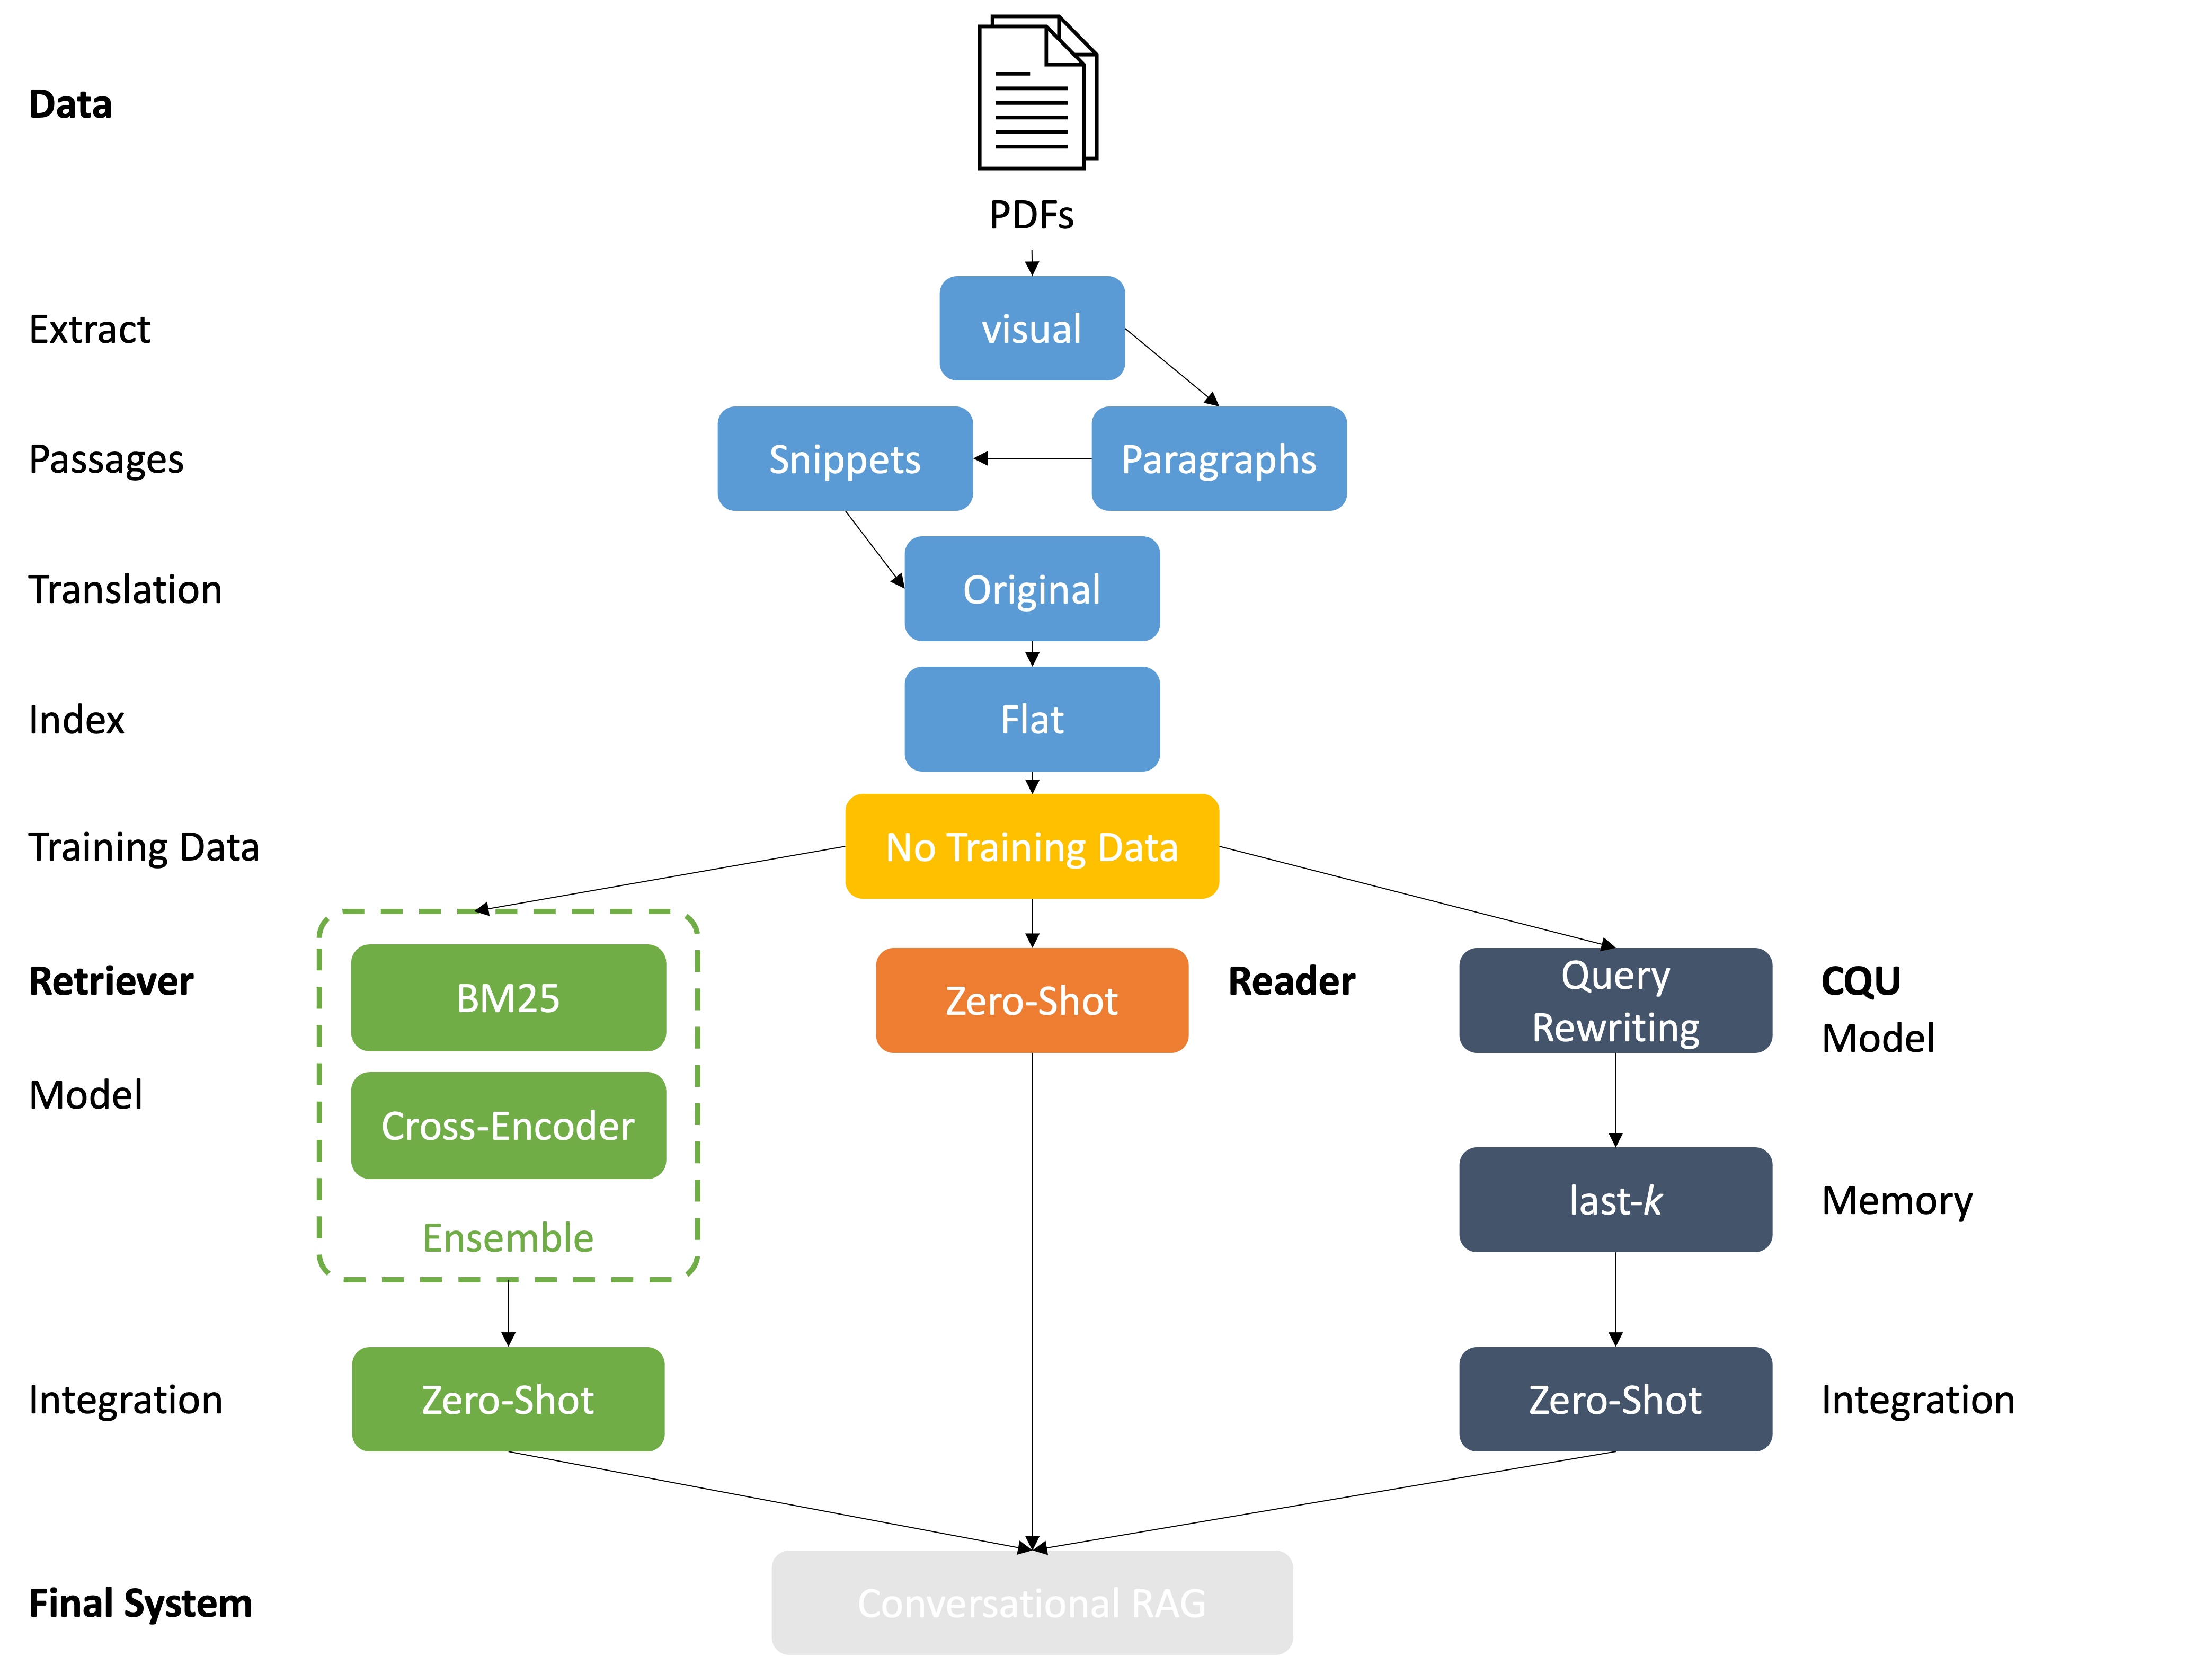
\includegraphics[width=\textwidth]{Grafiken/example_decission_tree.png}
%     \caption{Example of applying the Framework to a System Implementation}
%     \label{fig:example_decission_tree}
% \end{figure}



\subsection{extract}
\label{subsec:extract}

The sub-task of \textit{Inforamtion Extraction} was defined in the previous Section as sub-task (1) of the model $M$. Given a set of documents $D$, the knowledge source $P$ needs to be extracted using \textit{Information Extraction} techniques in combination with \textit{Passage Extraction} operations. As synthetic data generation is also part of the extraction component according to Section \ref{sec:overview}, it will also be discussed in this section. This is originally not part of the model $M$, but makes from a system architecture sense, to place these operations in this system component. Synthetic Data can be seen as an seperate task, which has nothing to do with the original task of \gls{convqa}, but is a necessary step in order to train components of the model $M$ or evaluate those.

\vspace{\baselineskip} % Add one line space

\textbf{Information Extraction:} When it comes to extracting text from any document $d$, there are many approaches to choose from. Some extract structures, metadata, or similar, which can be further utilized, while others extract unstructured text only. In any case, this extraction process highly depends on the source document type. An HTML website requires different approaches and tools compared to a PDF, for instance. An example tool for direct extraction of PDFs is Py2PDF \cite{noauthor_welcome_nodate}. Regardless of the source document and tool used to extract textual information $C_d$, there are two major possible outcomes given a set of documents $D$:

\begin{enumerate}
    \item \textit{Structured Extraction:} Denoted as $f_{StrucExt}(\cdot)$, in this extraction operation, $C_d$ can be extracted into logical segments directly: $f_{StrucExt}(d) = \{c_{d_i} \subseteq C_d : i \in \{1, 2, \ldots, n\}, C_d = \bigcup_{i=1}^{n} c_{d_i}\}$. If $f_StrucExt$ is applied to all documents $d$ in $D$, the resulting set $C$ contains all the outputs of $f_{StrucExt}$ for each document in $D$. Formally, $f_{StrucExt}(D) := C = \{C_{d_1}, C_{d_2}, \dots, C_{d_m}\}$, where each document $d$ is transformed into a set of logical segments $C_{d_i}$ representing its content.
    \item \textit{Unstructured Extraction:} Denoted as $f_{UnstExt}(\cdot)$, when applied to $D$, it results in a concatenated text corpus $C_d = \{c_d\} $ containing the textual content of a document $d$: $f_{UnstExt}(D) := C = \{C_{d_1}, C_{d_2}, \dots, C_{d_n}\}$, where each document $d$ is transformed into a single text snippet $c_d$ representing its content.
\end{enumerate}

In order to generate now snippets $p$ from $C$, \textit{Passage Extraction} has to be applied on $C$.

\vspace{\baselineskip} % Add one line space

\noindent\textbf{Passage Extraction:} The implementation of passage splitting depends on the nature of $C$ and the desired granularity of the output. In general, there are three operations for constructing passages $p$ based on a text snippet $c_d$:

\begin{enumerate}
    \item \textit{Paragraphs:} $f_p(\cdot)$ is an operation that transforms a collection $C_d$ of texts $c_d$ into a set of passages $P = \{p_1, p_2, \dots, p_n\}$. It operates similarly to $f_{StrucExt}(\cdot)$, but instead of $D$, it operates on $C_d$. The output of $f_p(\cdot)$ consists of passages $p$ that represent logical segments of the text corpus $c_d$. Usually, it operates in a \textit{rule-based} manner, meaning that a paragraph is defined by a token indicating a paragraph (e.g., \textit{<p/>} in HTML). The length $l$ of each $p_i$ is variable, and the number of paragraphs $|P|$ can also vary.
    \item \textit{Snippets:} $f_s(\cdot)$, when you have a fixed passage length $l$, divides the concatenated text $c_d$ into $|c_d|\bmod{l} + 1$ passages $p$ per $c_p$. Alternative approaches may involve specifying minimum and maximum lengths, denoted as $l_{\text{min}}$ and $l_{\text{max}}$. The exact point of division depends on whether a sentence ends within the specified window or not. If a sentence ending is found within the window, the snippet concludes at that point. Otherwise, it concludes at the end of the window. The individual length of the extracted passages $P = \{p_1, p_2, \ldots, p_n\}$ is not fixed in the case of syntactic snippets, as well as the number of paragraphs $|P|$.
    \item \textit{Sliding Windows:} $f_w(\cdot)$ utilizes a window size $l$, a concatenated text $c_d$, and a step size $s$. The window slides over the text $c_d$, and the text within the window is used as a passage $p$. This results in $\frac{|c_d| - l}{s}$ passages, denoted as $P = \{p_1, p_2, \ldots, p_n\}$.
\end{enumerate}

These operations can be combined in a pipeline fashion. For example, first $f_p(C_d) := P_{paragraphs} = \{p_{paragraphs,1}, p_{paragraphs,2}, \dots, p_{paragraphs,n}\}$ is constructed, and afterwards, on the logical paragraphs, $f_w(f_p(C_d)) := f_w(P_{paragraph}) = P_{window} = \{p_{window,1}, \allowbreak p_{window,2}, \allowbreak \dots, p_{window,i}\}$ is applied. The way these operations are combined is highly use-case specific and needs to be evaluated for each use-case individually. Another important factor influencing the decision regarding the parameters $l$ and, in general, the operation used, is the desired model for the \textit{Retriever} and \textit{Reader} as they may be trained on a specific token length as input or have a maximum length of tokens they accept as input or require a certain clarity of data points.


\vspace{\baselineskip} % Add one line space
\noindent\textbf{Synthetic Training Data Generation:} This can be interpreted as a knowledge distillation task. The main idea is to use a model $ED(\cdot)$ to generate a synthetic dataset for the sub-task and problem field of \textit{Passage Retrieval} and \textit{Response Generation}:

\begin{equation}
    \mathbf{ED(P) := (P, Q, I)}
    \label{eq:task}
\end{equation}

Where $P = \{p_1, p_2, \dots, p_n\}$ corresponds to a corpus of passages to retrieve from, $Q$ is a set of questions, and $I$ is the underlying search intent for a question $q \in Q$. If $I(q,p) = 1$, this means that the passage reflects the question's search intent. Given this task, there are several synthetic dataset types:

\begin{enumerate}
    \item \textit{Questions given Context} $ED_{qgp}(p,I) := q_s$: Given a passage $p$, generate a synthetic question $q_s$ that satisfies the desired search intent $I$. Applying $ED_{qgp}(P)$ to a set of passages will generate a set of questions $Q_s = \{q_1, q_2, \dots, q_n\}$, with one question for every passage, i.e., $|Q_s| = |P|$. $ED_{gpq}$ can also be applied multiple times with different $i \in I$ to generate multiple different questions $q_{j,s,1}, q_{j,s,2}, \dots , q_{j,s,i}$ for a single passage $p_j$.
    \item \textit{Question-Context-Answer Triples} $ED_{qpa}(p, I) := (q_s, p, a_s, I)$: Given a passage $p$, generate a synthetic question $q_s$ that satisfies the search intent $I$ and provides an answer $a_s$, where $I(q_s, a_s, p) = 1$. The result of applying $ED_{qpa}(P)$ to a set of passages is a set of question-passage-answer triples $QPA_s = \allowbreak \{(q_{1,s}, p_1, a_{1,s}, I), \allowbreak (q_{2,s}, p_2, a_{2,s}, I), \allowbreak \dots, (q_{n,s}, p_n, a_{n,s}, I)\}$, where $|QPA_s| = |P|$. $ED_{qpa}$ can also be applied multiple times with different $i \in I$ to generate multiple different questions $q_{j,s,1}, \allowbreak q_{j,s,2}, \dots , q_{j,s,i}$ and corresponding answers $a_{j,s,1}, \allowbreak a_{j,s,2}, \dots , a_{j,s,i}$ for a single passage $p_j$.
\end{enumerate}

While the previous two approaches focus on single tuples of either $(q,p)$ or triples of $(q,p,a)$, there is also a problem field of generating conversations based on passages $P = \{p_1, p_2, \dots, p_n\}$ from the same underlying document $d$. Therefore, the task given in Equation \ref{eq:task} is changed to:

\begin{equation}
    \mathbf{ED(P) := (H, P, I)}
    \label{eq:task_conversation}
\end{equation}

Where $H$ corresponds to a set of conversation histories $h$ containing multiple turns. The first turn is always a question $q_1$, followed by an answer $a_1$ based on a passage $p \in P$, also given a search intent $I$ over the whole history $h$. Synthetic datasets for this task can be generated in the following ways:

\begin{enumerate}
    \setcounter{enumi}{2} % Set the starting value to 3
    \item \textit{Conversational Question-Context-Answer Histories} $ED_{cqpa}(E, I) := H_s$: Given a subset of passages $E \subset P$, the task of the model $ED_{cqpa}$ is it to construct a realistic conversation with an intent $I$ over the corpus $E$. The result of applying $ED_{cqpa}(E,I)$ on a set of passages is a set of conversation histories $H_s = \{h_1, h_2, \dots, h_n\}$. $ED_{cqpa}$ can also be applied multiple times with different $i \in I$ in order to generate multiple different conversations $h_{j,s,1}, h_{j,s,2} \dots , h_{j,s,i}$ for a single subset of passages $E \subset P$.
\end{enumerate}

There are several ways to implemnt the models $ED_{qgp}$, $ED{qpa}$ or $ED_{cqpa}$. Implementations of those appraoches will be discussed in Chapter \ref{chap:eval}. 


% In this pipeline, the prompt-based \gls{qg} method known as PROMPTAGATOR \cite{dai_promptagator_2022} is used to generate a synthetic \gls{qa} dataset for ColBERTv2 \cite{santhanam_colbertv2_2022} based on $P$. The goal is to create triples of $(q, p^{+}, p^{-})$, similar to those found in datasets like MS MACRO \cite{bajaj_ms_2018}. For the task of $E_{qg}(p) := q$, a \gls{s2s} model, specifically a \gls{llm}, will be employed. This technique can be interpreted as knowledge distilation from the LLM to the later trained retriever. Similar to PROMPTAGATOR, there are two approaches to consider:

% \begin{enumerate}
%     \item \textit{Zero-Shot:} In this approach, a single prompt is executed to generate a question $q_i$ corresponding to a passage $p_i$, all without the need for any supervised dataset.
    
%     \item \textit{Few-Shot:} This approach uses $k$ supervised pairs $(q_j, p^{+}_{j})^{k}$ to generate a question $q_i$ corresponding to a passage $p_i \in P$.
% \end{enumerate}

% The prompt used for \textbf{zero-shot \gls{qg}}, where $p_i$ represents a passage from $P$, is:

% \verb|f'{p_i} Read the passage and generate a corresponding query.'|

% The prompt used for \textbf{few-shot \gls{qg}}, where $q_j$ represents a question, $p_j$ the corresponding passage, and $p$ the passage for which a question is being generated, is:

% \verb|f'Passage: {p_1} Question: {q_1} XXX Passage: {p_2} Question: {q_2}|

% \verb|XXX ... XXX Passage: {p} Question:'|

% The result of either of these approaches will be a synthetic training dataset of $(q_s, p^{+})$ tuples. This dataset can be used for fine-tuning the retriever.

% A major issue associated with this form of \textbf{\gls{qg}} is its strict limitation to extractive questions, where the evidence can be derived from a single passage only. This limitation significantly constrains this pipeline. However, it does not necessarily prevent the system from answering more complex questions, such as multi-hop questions. These can be addressed by the \textit{retriever} and \textit{reader} modules.



\subsection{Retriever}
\label{subsec:retriever}

\subsection{Reader}
\label{subsec:reader}

\subsection{Contextual Query Understanding}
\label{subsec:cqu}


% \section{Question Answering over PDFs}
% \label{sec:qa-over-pdfs}

% \begin{figure}
%     \centering
%     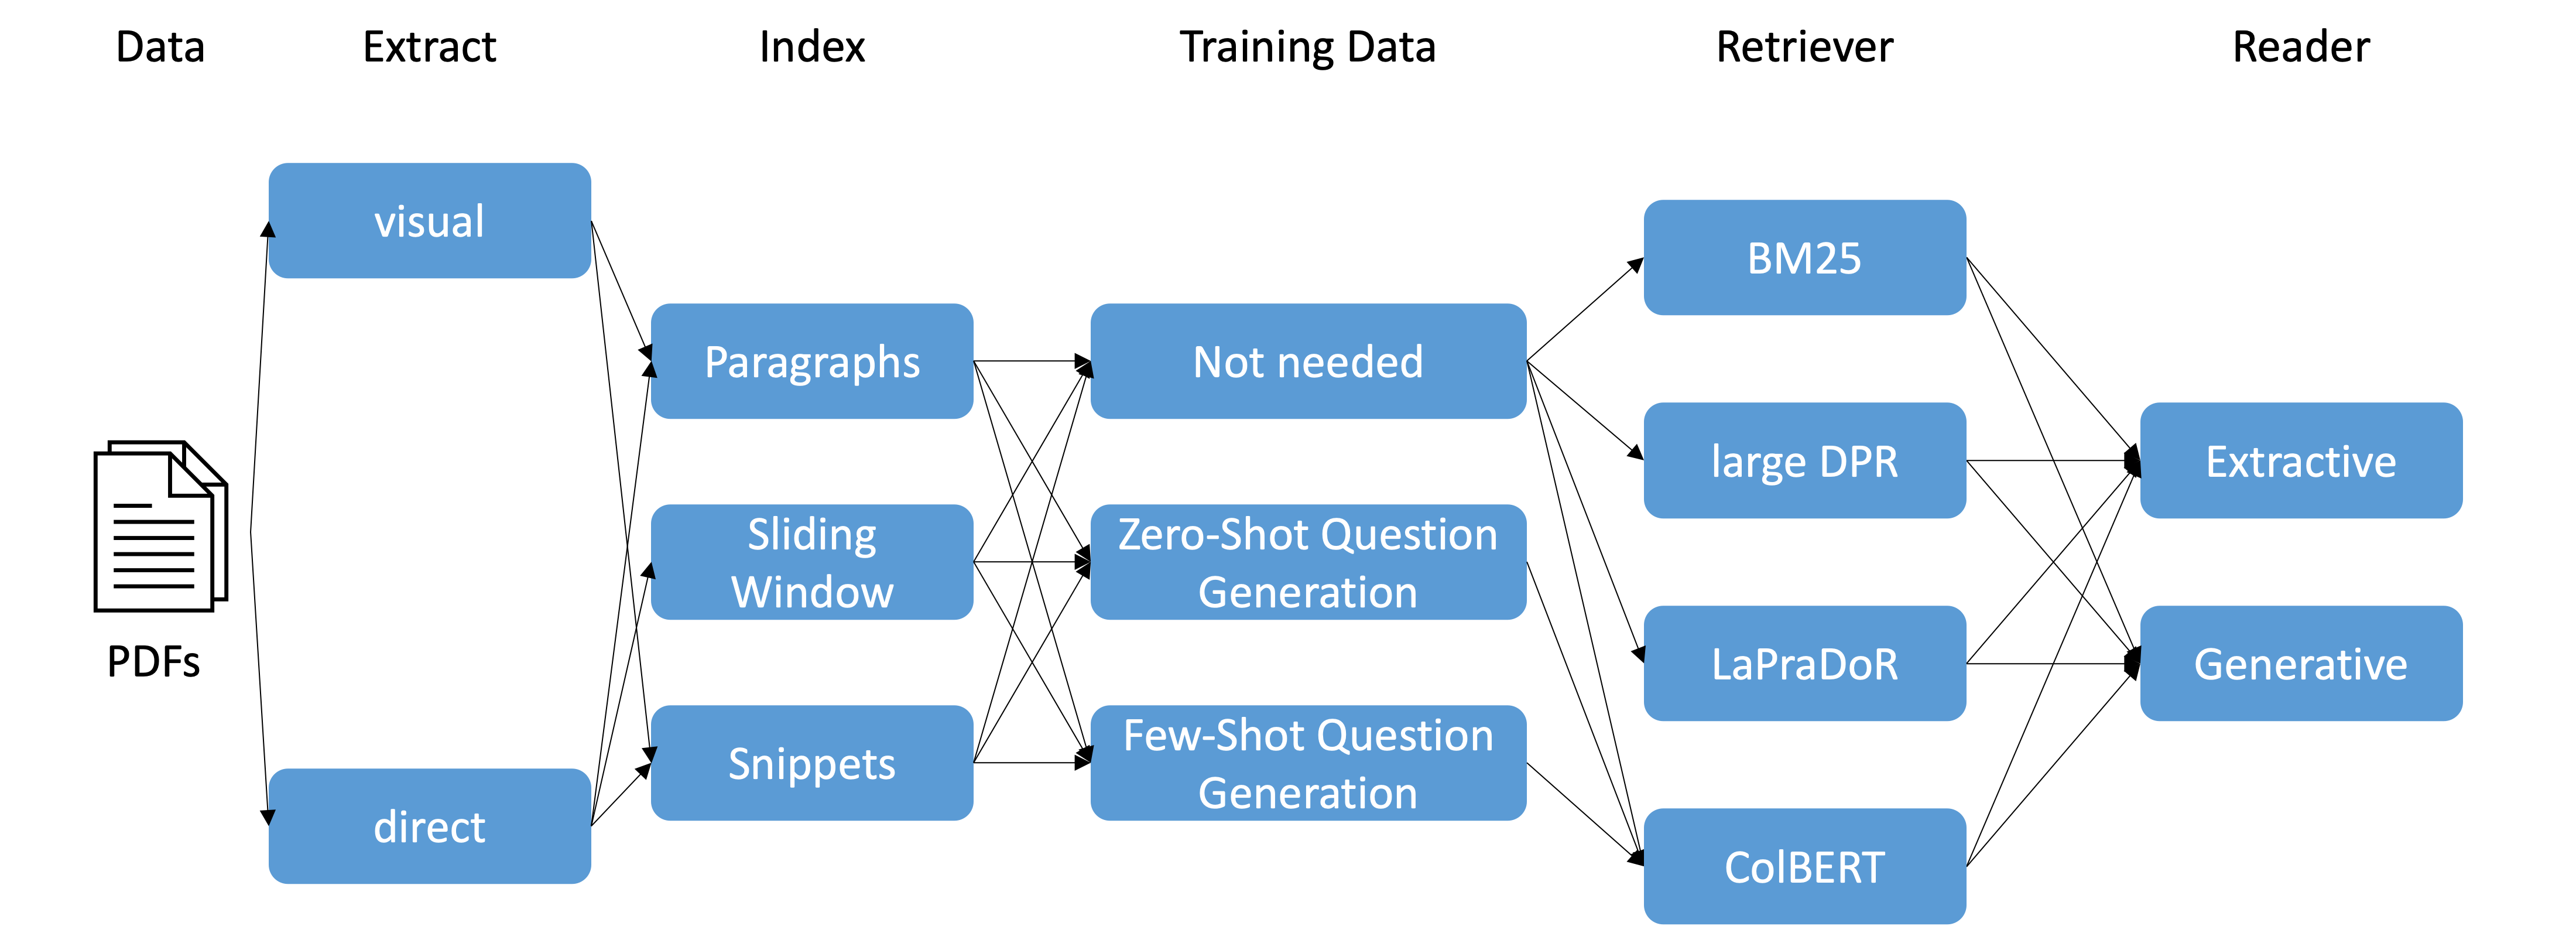
\includegraphics[width=0.8\textwidth]{Grafiken/Possible_Systems.png}
%     \caption{Possible Combinations of Modules to Create an Adapted QA-System}
%     \label{fig:qa-system-combinations}
% \end{figure}

% The possible combinations of modules to create an adapted \gls{qa}-System can be seen in Figure \ref{fig:qa-system-combinations}.


% \subsection{Extract}
% \label{subsec:extract}
% %%%%%

% \subsection{Retrieve}
% \label{subsec:retrieve}

% \textbf{Out-of-Domain Retrievers:} The easiest implementation is the out-of-domain usage of retrievers without fine-tuning and the need for generating a training dataset. Three major retrievers seem promising due to their performance on the BEIR \cite{thakur_beir_2021} out-of-domain benchmark for retrievers:

% \begin{enumerate}
%     \item \textit{BM25} is the standard Sparse Retriever based on lexical probabilistic matching between the query $q$ and passages $p$.
%     \item \textit{Large DPRs} are Dense Retrievers based on large encoders. They utilize typical dense retrieval paradigms and are a primary approach in open-source projects like \textit{Langchain} \cite{noauthor_langchain-ailangchain_nodate}.
%     \item \textit{LaPraDoR} is a hybrid retriever based on a broadly trained Representation-based Retriever, similar to (2), combined with lexical weighting (1).
% \end{enumerate}

% The \gls{laprador} utilizes the advantages of both lexical and semantic search. Given a question $q$ and a passage $p$, the semantic similarity $\text{sim}(q,d)$ is calculated using a \gls{dpr} model. In addition, the lexical similarity $\text{BM25}(q,d)$ is calculated. The final score $\text{score}(q,d)$ is computed as follows:

% \begin{equation}
%     \mathbf{score}(q, d) = \mathbf{sim}(q, d) \cdot \mathbf{BM25}(q, d)
% \end{equation}

% This approach achieves state-of-the-art performance on the BEIR benchmark without the need for fine-tuning. It serves as the ideal off-the-shelf component for the desired \gls{qa}-System.

% \noindent\textbf{Fine-Tuning Retrievers:} Fine-tuning is a challenging task in the absence of a supervised dataset, especially when dealing with a Representation-Interaction Retriever like ColBERTv2. Currently, there is no clear reference on how to fine-tune a Representation-Interaction Retriever like ColBERTv2 on synthetic data. To address this gap, this thesis proposes the approach depicted in Figure \ref{fig:retriever-fine-tuning}, which combines elements from the training processes of PROMPTAGATOR \cite{dai_promptagator_2022}, the original \gls{dpr} \cite{karpukhin_dense_2020}, and ColBERTv2 \cite{santhanam_colbertv2_2022}.

% \begin{figure}
%    \centering
%     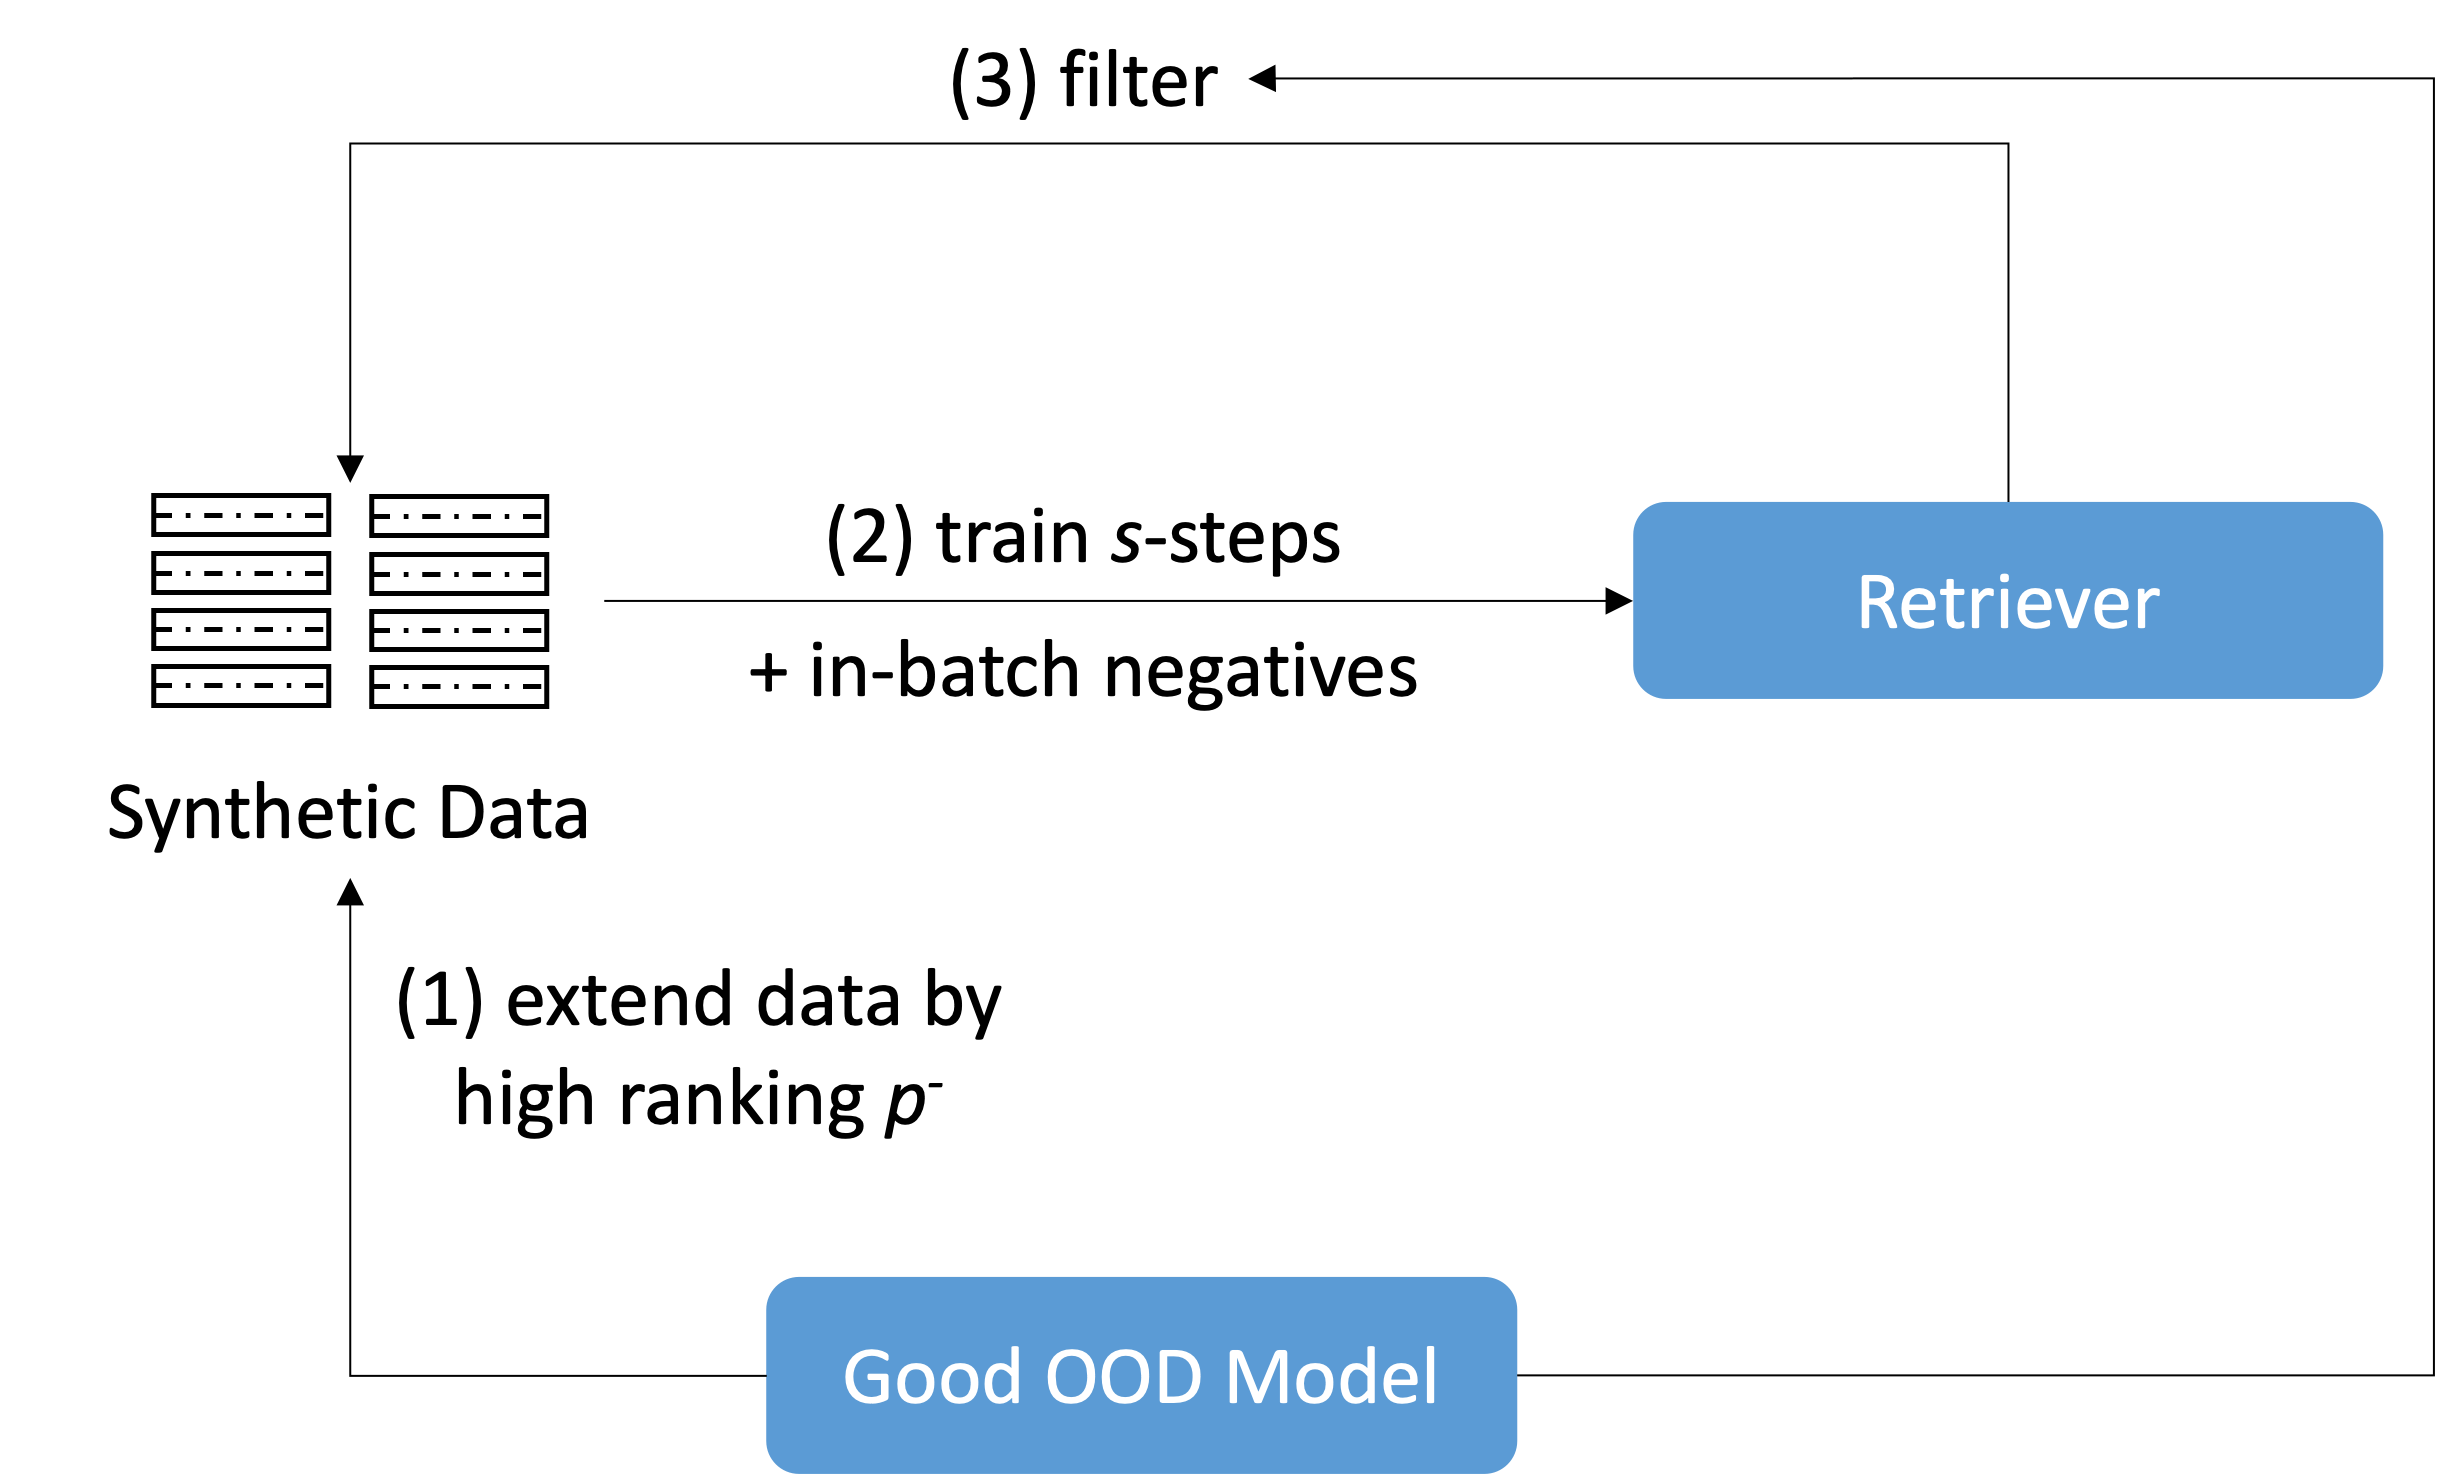
\includegraphics[width=0.8\textwidth]{Grafiken/Training.png}
%     \caption{Fine-Tuning Process for Retriever}
%     \label{fig:retriever-fine-tuning} 
% \end{figure}

% A crucial aspect of this fine-tuning approach is the utilization of an already well-performing out-of-domain retriever as a baseline. This baseline retriever can distill its knowledge into the retriever undergoing training. For example, \gls{dpr} used BM25, while ColBERTv2 employed MiniLM \cite{wang_multi-passage_2019}, a 22M-parameter Interaction-based retriever. A useful guideline for selecting the model is to consult the BEIR leaderboard.

% In the first step, the \gls{ood} model must retrieve the top $k$ passages, denoted as $p_i$, for each synthetic $(q_s,p^{+})$ pair. To generate numerous high-quality negative triples, denoted as $(q_s, p^{+}, p^{-})$, for every retrieved passage $p_i$ (where $p_i \neq p^{+}$), the triple $(q_s, p^{+}, p_i)$ is added to the training dataset.

% In the second step, the target retriever is trained for $s$ iterations. The loss function employed is the negative log likelihood, as defined in Section \ref{subsec:qa_retrieval}. During training, in-batch negatives are utilized. Let $Q$ and $P$ represent the $(B \times d)$ matrices of question and passage embeddings in a batch of size $B$. The matrix $S = Q P^{T}$ contains rows where each corresponds to a question paired with all other passages in the batch. The passages from all the other data points act as negatives for the question $q$.

% In the third step, the synthetic dataset is subjected to filtering. PROMPTAGATOR demonstrated promising results of filtering data by a network trained on the data. For this filtering process, retrieval is performed using both the newly trained model and the \gls{ood} model for a question $q_s$. If neither model retrieves the corresponding passage $p^{+}$ for the synthetic question within their top $k$, that question is removed from the dataset.

% Steps two and three are repeated once during fine-tuning.
% \subsection{Read}
% \label{subsec:read}

% \textbf{Out-of-Domain Readers:} There exists no benchmark for the application of zero-shot or \gls{ood} Readers. As Pereira et. al. \cite{pereira_visconde_2022} point out in their experimental results, the zero-shot performance of \gls{llm}s as Generative Readers is state-of-the-art and thus needs no fine-tuning and can even perform in a zero-shot setting. Luo et. al. \cite{luo_choose_2022} also pointed out, that the \gls{ood} performance of Extractive Readers is higher than the of Generative ones, when it comes to \gls{prlm}. Threfore a good \gls{ood} model choice is UnifiedQA-v2 \cite{khashabi_unifiedqa-v2_2022}, which is based on T5 \cite{raffel_exploring_2023} and was trained on 20 diverse datasets.

% \noindent\textbf{Fine-Tuning Readers:} Extractive Readers depend on datasets of the form $(q, c, a_span)$, whereas $q$ is a question, $c$ the context and $a_span$ an indication of which tokens of $c$ correspond to the desired answer. Similar for Generative Readers, which need $(q, c, a)$ datasets, whreas $a$ is just a text based answer to question $q$. The training process for the reader is easier and more straightforward as for the retriever. Given the already filtered synthetic trainings dataset, this can be used for training of the reader.

% \subsection{Orchestration}
% \label{subsec:qa_orchestration}

% Similar to \gls{r2d2}\cite{fajcik_r2-d2_2021} and LaPraDoR \cite{xu_laprador_2022} and others, an orchestration of retrievers and readers will be adopted in order to achieve highest \gls{ood} performance. This involves the following steps:

% \begin{enumerate}
%     \item \textit{Retrieval:} The $k$-top identified passages $P = \{p_1, p_2, \ldots, p_k\}$ are retrieved for a given question $q$ receive a similarity indication $\text{sim}(q,p_k)$ by the retriever. Next to this score, the BM25 score is calculated $BM25(q,p_k)$. The final score is calculated as the weighting of the similarity by BM25:     $score(q, d) = sim(q, d) \cdot BM25(q, d)$
%     \item \textit{Reader:} As for the Reader two readers will be executed at the same time: An extractive and one generative reader. Both 

% \end{enumerate}


% \section{Conversational Question Answering System}
% \label{sec:conv-qa-system}